

\section{Introduction}

The GARCH family of models (Bollerslev, 1986) remains the workhorse for daily volatility forecasting in financial markets. A substantial literature has developed around asymmetric extensions---most notably the GJR-GARCH of Glosten, Jagannathan, and Runkle (1993) and the EGARCH of Nelson (1991)---designed to capture the empirical observation that negative equity returns tend to increase future volatility more than positive returns of equal magnitude. This ''leverage effect,'' first noted by Black (1976) and formalized by Christie (1982), is well-documented for equity markets and has become a standard consideration in volatility model specification.

However, the implicit assumption in much of the applied GARCH literature---that asymmetric models uniformly improve upon their symmetric counterparts---warrants closer examination when moving beyond equities. While Chevallier and Ielpo (2017) document inverted asymmetric volatility in gold and several agricultural commodities, the implications of this reversal for model selection, risk management, and portfolio construction have not been systematically explored.

This paper makes three contributions to the volatility forecasting and financial risk management literature.

\textbf{First}, we propose a leverage direction taxonomy based on the GJR-GARCH $\gamma$ parameter across seven primary assets spanning equities (SPY, QQQ, EEM), precious metals (GLD, SLV), government bonds (TLT), and cryptocurrency (BTC-USD), validated on up to 26 assets. The sign of $\gamma$ corresponds to the asset's price-driving mechanism: risk assets exhibit standard leverage ($\gamma > 0$), safe-haven assets show inverted leverage ($\gamma < 0$), and interest rate instruments display no significant asymmetry ($\gamma \approx 0$). Gold's inverted leverage is statistically significant (HAC $t = -5.79$, $p < 0.001$) and persists across 93\% of quarterly estimation windows. Notably, gold's leverage direction is regime-dependent---inverted during fear-driven rallies but standard during liquidation-driven declines ($t = -4.71$, $p < 0.0001$ for the regime difference). This taxonomy determines optimal GARCH specification: GJR-GARCH significantly outperforms symmetric GARCH only when $\gamma > 0.10$, correctly classifying all twelve Diebold-Mariano comparisons across two out-of-sample periods. We propose that $\gamma$ direction, rather than the commonly used return skewness, provides a more reliable model selection criterion.

\textbf{Second}, we link leverage direction to the economic channel through which volatility targeting (VT) generates alpha, generalizing the equity-specific finding of Hood and Raughtigan (2025). Within equity-type assets, $\gamma$ predicts whether VT acts as trend-following or contrarian (Spearman $\rho = 0.886$, $p = 0.019$ for six assets), with out-of-sample predictive power ($\rho = 0.821$ using $\gamma$ from 2010--2017 to predict trend beta in 2018--2026). However, this relationship does not extend to diverse asset classes ($\rho = -0.448$, $p = 0.14$ for twelve assets), delineating the proposition's domain. Meanwhile, VT's primary benefit---maximum drawdown reduction---is universal across all twelve tested assets and driven by base volatility level ($\rho = 0.944$, $p < 0.001$), independent of $\gamma$.

\textbf{Third}, we document persistent time-zone information transmission in which U.S.\ market information spills over to Asian equity markets with a one-day delay. % Codex-R6-fix: reframed from "tradable alpha" to "information transmission evidence"
A simple momentum strategy---holding the local index when trailing SPY returns are positive, otherwise cash---achieves $t$-statistics exceeding the \citet{harvey2016} multiple-testing threshold of 3.0 in six Asia-Pacific markets using close-to-close returns: Hong Kong ($t = 4.12$), Australia ($t = 4.04$), Singapore ($t = 4.03$), Korea ($t = 3.83$), Taiwan ($t = 3.75$), and Japan ($t = 3.69$), after transaction costs. A global portfolio combining U.S.\ volatility targeting and Asian time-zone momentum achieves a c2c Sharpe of 1.61 ($t = 4.31$) with maximum drawdown of $-8.4\%$; however, this represents an upper bound, as approximately 78\% of the c2c alpha is attributable to overnight gaps that are not capturable by implementable open-to-open execution (Appendix~\ref{sec:tz_arbitrage}). The c2c results are best interpreted as evidence of information transmission speed rather than achievable trading returns.

Supporting findings reinforce a broader pattern: increasing model sophistication improves statistical measurement but not investable allocation decisions. The Student-$t$ distributional correction reduces VaR violations by 21--48\%, but more complex approaches (DCC-GARCH, copula, GARCH-MIDAS, Markov-switching) provide negligible additional improvement to portfolio allocation.

The remainder of the paper is organized as follows. Section 2 reviews the relevant literature on GARCH modeling, leverage effects, VaR backtesting, and volatility targeting. Section 3 describes our data and methodology. Section 4 presents empirical results. Section 5 discusses implications and limitations. Section 6 concludes.



\section{Literature Review}

\subsection{GARCH Models and the Leverage Effect}

Bollerslev's (1986) GARCH model captures the well-documented volatility clustering in financial returns but assumes symmetric responses to positive and negative innovations. The observation that equity volatility tends to rise more following negative returns---the ''leverage effect'' first noted by Black (1976) and attributed to changes in financial leverage by Christie (1982)---motivated asymmetric extensions.

Nelson (1991) introduced the Exponential GARCH (EGARCH), modeling the logarithm of conditional variance with separate coefficients for the sign and magnitude of innovations. Glosten, Jagannathan, and Runkle (1993) proposed the GJR-GARCH, adding an indicator function for negative innovations. Both models have become standard tools in applied finance, with Engle and Siriwardane (2018) providing a structural interpretation linking the GJR gamma parameter to firms' capital structure dynamics.

Empirically, asymmetric GARCH models generally improve upon symmetric specifications for equity indices (see Hansen and Lunde, 2005, for a comprehensive comparison of 330 GARCH variants). However, the question of whether this improvement extends to non-equity asset classes has received less systematic attention.

\subsection{Commodity Volatility and Inverted Asymmetry}

The behavior of volatility in commodity markets differs from equities in important ways. Chevallier and Ielpo (2017) investigate the leverage effect across a broad set of commodities and find that gold, wheat, coffee, and cocoa exhibit inverted asymmetric volatility---where positive price shocks increase volatility more than negative shocks. This is consistent with earlier findings for specific commodities (e.g., Batten, Ciner, and Lucey, 2010, for precious metals).

The economic interpretation differs from equities: while equity leverage operates through capital structure, commodity price increases during stress periods reflect uncertainty about supply, demand, or financial conditions. For gold specifically, Baur and McDermott (2010) and Baur and Lucey (2010) establish that gold functions as both a hedge and a safe haven for developed market equities, with its hedging effectiveness increasing during extreme market downturns.

More recently, Chang, Chen, Kung, and Tian (2021) use a Markov-switching GJR-GARCH model to link gold's inverted asymmetry to high-volatility regimes, showing that gold's safe-haven ability is concentrated in these regimes. This finding aligns with our regime-dependent leverage result, though our analysis extends to a broader asset class framework and examines the implications for model selection, VaR compliance, and portfolio construction---dimensions not addressed in the existing literature.

\subsection{Value-at-Risk and Basel III}

The Basel Committee's internal models approach (BCBS, 2006, 2019) requires banks to backtest their VaR models against realized losses. Kupiec (1995) provides the unconditional coverage test, while Christoffersen (1998) adds the independence dimension. McNeil, Frey, and Embrechts (2015) provide a comprehensive treatment of quantitative risk management methodology.

The choice of distributional assumption is known to significantly impact VaR accuracy. Bollerslev (1987) introduced Student-t innovations for GARCH models, and subsequent work (e.g., Hansen, 1994) developed skewed-t and other flexible distributions. Kuester, Mittnik, and Paolella (2006) find that GARCH models with appropriate distributional assumptions outperform historical simulation and extreme value approaches for VaR estimation.

\subsection{Volatility Targeting}

Moreira and Muir (2017) demonstrate that scaling portfolio exposure by the inverse of conditional variance---volatility targeting---generates significant alphas across equity market factors, value, momentum, and currency carry. Their key insight is that changes in volatility are not offset by proportional changes in expected returns, creating a risk-return tradeoff that VT can exploit.

Harvey, Hoyle, Korgaonkar, Rattray, Sargaison, and Van Hemert (2018) extend these results to multi-asset portfolios. Fleming, Kirby, and Ostdiek (2001, 2003) provide earlier evidence that volatility timing improves portfolio performance. Hood and Raughtigan (2025) demonstrate that VT alpha for equities arises primarily from implicit trend-following via the leverage effect: because negative returns raise volatility and trigger deleveraging, VT mechanically reduces exposure after declines---an effect that is equity-specific and absent in assets without standard leverage. This insight connects to our gamma taxonomy, as the direction of this implicit trend-following reverses for inverted-leverage assets.

More recently, Cederburg et al. (2020) demonstrate that using VIX as the scaling signal---exploiting the forward-looking nature of implied volatility---produces an alpha of approximately 4.9\% for equity portfolios, compared to realized-variance scaling. Bozovic (2024) extends this finding by showing that VIX-based strategies generally dominate realized-volatility-based alternatives, attributing the advantage to VIX's incorporation of forward-looking option-market information. DeMiguel, Martin-Utrera, and Uppal (2024) formalize this integration by combining historical and implied volatility in a multifactor framework, achieving a 13\% improvement in out-of-sample Sharpe ratios---providing theoretical support for hybrid approaches that blend realized and implied information. Xu (2024) demonstrates the real-time viability of volatility-managed portfolios, finding that 148 out of 197 equity factors are improved in real time after accounting for estimation error and transaction costs.

However, the effectiveness of VT across different leverage regimes---particularly for assets with inverted leverage---has not been previously examined, nor has the interaction between VIX- and GARCH-based signals been formalized through a principled switching mechanism that integrates implied and realized information for variance management.

\subsection{Deep Learning for Volatility Forecasting}

Recent work has explored neural network approaches to volatility forecasting. Hybrid GARCH-LSTM models (e.g., Kim and Kim, 2019; Araya et al., 2024) attempt to combine the structural advantages of GARCH with the flexibility of deep learning. However, the incremental improvement over well-specified GARCH models remains debated, particularly at daily frequency where GARCH models may already extract the available signal in squared returns (see Bucci, 2020, for a skeptical assessment).



\section{Data and Methodology}

\subsection{Data}

We use daily adjusted closing prices for seven exchange-traded assets: SPDR S\&P 500 ETF Trust (SPY), Invesco QQQ Trust (QQQ), iShares MSCI Emerging Markets ETF (EEM), SPDR Gold Shares (GLD), iShares Silver Trust (SLV), iShares 20+ Year Treasury Bond ETF (TLT), and Bitcoin (BTC-USD). Data are sourced from Yahoo Finance for the period January 2017 through March 2026. % Codex-R6-fix: date range unified to match extended OOS (was "December 2025") For U.S.-listed ETFs, Yahoo Finance prices reflect official exchange data with corporate action adjustments; we verify price accuracy against Bloomberg terminal data for key crisis dates (COVID crash, March 2020; Iran crisis, March 2026) and find no discrepancies. Daily returns are computed as simple percentage changes $r_t = (P_t - P_{t-1})/P_{t-1}$.

Table 1 reports descriptive statistics. All return series reject normality (Jarque-Bera p < 0.001), exhibit significant ARCH effects (Engle's LM test p < 0.001), and are stationary (ADF p < 0.001). Excess kurtosis ranges from 3.52 (GLD) to 14.61 (SPY), motivating the consideration of fat-tailed distributions for VaR estimation.

\subsection{Volatility Models}

We consider two specifications from the GARCH(1,1) family:

\textbf{GARCH(1,1):}
\begin{equation}
\sigma^2_t = \omega + \alpha \varepsilon^2_{t-1} + \beta \sigma^2_{t-1}
\end{equation}

\textbf{GJR-GARCH(1,1)} (Glosten et al., 1993):
\begin{equation}
\sigma^2_t = \omega + (\alpha + \gamma \mathbf{1}_{\varepsilon_{t-1}<0}) \varepsilon^2_{t-1} + \beta \sigma^2_{t-1}
\end{equation}

where $\gamma$ captures the asymmetric response to positive versus negative innovations. When $\gamma > 0$, negative returns produce higher conditional variance (standard leverage effect). When $\gamma < 0$, positive returns increase variance (inverted leverage).

All models are estimated with zero-mean specification and Normal distribution using the \texttt{arch} package in Python (Sheppard, 2023). For VaR applications, we additionally consider Student-t distributed innovations with estimated degrees of freedom.

\subsection{Rolling Estimation}

We employ a rolling window approach with re-estimation at each forecast origin. The primary window size is $w = 504$ trading days (approximately 2 calendar years), which satisfies the minimum sample size recommendation for GARCH estimation ($\geq 500$ observations; see Hwang \& Valls Pereira, 2006) while avoiding contamination from distant regime changes. Robustness checks with $w \in \{252, 1000, 2000, 3000, 5000\}$ (Table~\ref{tab:window}) confirm that QLIKE rankings are qualitatively robust to window choice, though $w = 504$ produces the best QLIKE during high-volatility periods (2020--2021) while larger windows ($w \geq 2000$) perform marginally better during calm periods (2023--2024). The gamma sign classification is invariant to window size across all tested values.

For each out-of-sample date $t$, we estimate the model using data from $t-w$ to $t-1$, and produce a one-step-ahead variance forecast $\hat{\sigma}^2_t$. The realized variance proxy is the squared daily return $r^2_t$.

\subsection{Evaluation Criteria}

\subsubsection{Statistical Loss Functions}

The primary evaluation metric is the QLIKE loss function (Patton, 2011):
\begin{equation}
\text{QLIKE} = \frac{1}{T} \sum_{t=1}^{T} \left( \frac{r^2_t}{\hat{\sigma}^2_t} + \ln \hat{\sigma}^2_t \right)
\end{equation}

QLIKE is robust to noise in the realized variance proxy and ranks forecasts consistently regardless of the proxy used, provided the proxy has equal bias across models.

\subsubsection{Diebold-Mariano Test}

We test the null hypothesis of equal predictive accuracy between models using the Diebold-Mariano test (Diebold \& Mariano, 1995) with Newey-West HAC standard errors (5 lags):
\begin{equation}
DM = \frac{\bar{d}}{SE_{NW}(\bar{d})} \sim N(0,1)
\end{equation}
where $d_t = L(r^2_t, \hat{\sigma}^2_{1,t}) - L(r^2_t, \hat{\sigma}^2_{2,t})$ is the loss differential using QLIKE.

\subsubsection{VaR Backtesting}

Value-at-Risk at confidence level $\alpha$ is computed as:
\begin{itemize}
\item \textbf{Normal:} $\text{VaR}_\alpha = \Phi^{-1}(\alpha) \cdot \hat{\sigma}_t$
\item \textbf{Student-t:} $\text{VaR}_\alpha = t^{-1}_\nu(\alpha) \cdot \sqrt{(\nu-2)/\nu} \cdot \hat{\sigma}_t$

\end{itemize}
where $\nu$ is the degrees of freedom (fixed at 5 in our baseline, consistent with typical empirical estimates for financial returns). The choice of df = 5 is validated out-of-sample: Section~4.4 demonstrates that Basel III Green Zone compliance is achieved for all df $\leq$ 6, and that jointly estimating df produces \textit{worse} performance by over-adapting to quiet markets. The fixed df = 5 is thus a conservative choice that is robust across the empirical range df $\in$ [4, 7].

We apply Kupiec's (1995) unconditional coverage test (LR statistic, $\chi^{2}$ with 1 d.f.) and Christoffersen's (1998) independence test to assess violation clustering. Annual violation counts are classified per the Basel III traffic light system (Green: 0--4, Yellow: 5--9, Red: $\geq$10 violations per approximately 250 trading days).

\subsubsection{Leverage Direction Analysis}

To analyze the temporal stability of the leverage direction, we estimate GJR-GARCH on semi-overlapping quarterly windows (504-day windows advanced by 63 trading days) and collect the gamma estimates. % Codex-R6-fix: "non-overlapping" corrected to "semi-overlapping" to match Section 4 description We test:
\begin{itemize}
\item \textbf{H0:} $E[\gamma] \geq 0$ vs. \textbf{H1:} $E[\gamma] < 0$ (inverted leverage)
\end{itemize}
using a one-sided t-test on the quarterly gamma series.

\subsection{Volatility Targeting}

Following Moreira and Muir (2017), the volatility-managed portfolio weight is:

\begin{equation}
w_t = \frac{\sigma_{\text{target}}}{\hat{\sigma}_t}
\end{equation}

We set $\sigma_{\text{target}} = 10\%$ annualized for the GARCH-based analysis, and $\sigma_{\text{target}} = 12\%$ for the VIX-based analysis (Section~\ref{sec:ivt}), reflecting the VIX's systematic upward bias from the embedded variance risk premium. Weights are smoothed with a 5-day moving average and clipped to $[0, 1.5]$. Post-hoc transaction cost analysis (Section 5.1) confirms that the estimated annual turnover of 756\% generates cost drag of only 8--15 basis points at typical SPY bid-ask spreads.



\section{Empirical Results}

\subsection{Data Characteristics}

Table 1 summarizes the distributional properties of daily returns for our seven assets over 2017--2025. Several patterns inform our subsequent modeling choices.

All return series exhibit significant excess kurtosis, ranging from 3.52 (GLD) to 14.61 (SPY), and all decisively reject the normality hypothesis (Jarque-Bera p < 0.001). The ARCH LM test confirms significant conditional heteroskedasticity in all series (p < 0.001), justifying the application of GARCH-family models.

Return skewness varies across assets: SPY (-0.315), QQQ (-0.189), GLD (-0.296), and EEM (-0.584) all show negative skewness, while TLT (+0.155) and BTC-USD (-0.028) are approximately symmetric. A naive model selection approach based on skewness would suggest asymmetric GARCH models for all negatively skewed assets. As we demonstrate in Section 4.2, this criterion is misleading for gold: despite its negative skewness, gold's conditional variance responds asymmetrically to \textit{positive} shocks, not negative ones.

Annualized volatility spans an order of magnitude, from 14.6\% (GLD) to 57.3\% (BTC-USD). This range motivates our analysis of volatility targeting effectiveness as a function of base volatility level (Section 4.5).

The extreme minimum daily returns---SPY at -10.94\% (March 2020 COVID crash) and BTC-USD at -37.17\%---underscore the importance of fat-tailed distributions for VaR estimation, which we address in Section 4.4.


\subsection{Leverage Direction Across Asset Classes}

\subsubsection{Rolling Gamma Estimates}

We estimate the asymmetry parameter $\gamma$ of GJR-GARCH(1,1) using a rolling window of 504 trading days, updating quarterly. Table 2 reports the cross-sectional statistics of $\gamma$ for each asset.

The most striking finding is the \textbf{consistent sign difference across asset classes}. For equities (SPY, QQQ), $\gamma$ is uniformly positive across all quarterly estimates, indicating the well-documented leverage effect where negative returns amplify conditional variance. In contrast, gold (GLD) exhibits a \textbf{persistently negative $\gamma$}, with 93\% of quarterly estimates below zero (mean $\gamma$ = -0.067, std = 0.044). This inverted leverage effect---where \textit{positive} returns increase conditional variance---has not been documented in the prior GARCH literature as a systematic cross-asset phenomenon.

Treasury bonds (TLT) show near-zero $\gamma$ (mean = -0.008, std = 0.048), with approximately equal proportions of positive and negative estimates, indicating no significant asymmetry. Bitcoin (BTC-USD) displays mild standard leverage (mean $\gamma$ = +0.117), though with higher instability (std = 0.136) and occasional sign reversals.

\subsubsection{Economic Interpretation}

The inverted leverage effect in gold is consistent with gold's well-established role as a safe-haven asset (Baur \& McDermott, 2010; Baur \& Lucey, 2010). During periods of market stress, investors increase their allocation to gold, driving prices upward. This fear-driven buying creates heightened uncertainty about future gold prices, resulting in elevated conditional variance. Crucially, the mechanism operates in the opposite direction from the equity leverage effect (Black, 1976; Christie, 1982), where falling stock prices increase the debt-to-equity ratio and therefore firm risk.

The absence of leverage effects in Treasury bonds is likewise economically intuitive: bond price movements reflect interest rate changes, which do not systematically alter the issuer's (sovereign) credit risk in either direction.

\subsubsection{Implications for Model Selection}

Table 3 presents GARCH(1,1) versus GJR-GARCH(1,1) QLIKE comparisons across all asset-period combinations. The results reveal a clear pattern: GJR-GARCH significantly outperforms only when $\gamma$ is consistently positive and above approximately 0.10.

For SPY ($\gamma \approx$ +0.21), GJR achieves significantly lower QLIKE (DM test p = 0.001 for 2023--2024, p = 0.029 for 2025). For QQQ in 2025 ($\gamma \approx$ +0.17), GJR likewise wins significantly (p = 0.023). However, for GLD ($\gamma$ < 0), TLT ($\gamma \approx$ 0), and BTC-USD (mild $\gamma \approx$ +0.08), Diebold-Mariano tests fail to reject equal predictive accuracy at the 5\% level across all tested periods.

This finding has practical implications: the conventional approach of selecting asymmetric GARCH models based on return skewness can be misleading. GLD exhibits substantial negative skewness (-0.296) yet has inverted leverage---skewness-based model selection would incorrectly suggest GJR. We propose that \textbf{the sign and magnitude of the estimated $\gamma$ parameter} should replace skewness as the primary criterion for choosing between symmetric and asymmetric GARCH specifications.

\subsubsection{Robustness}

The $\gamma$ sign classification is robust to window size (results qualitatively identical with w = 252 and w = 756), estimation period (2007--2026 for SPY shows the same pattern), and model specification (EGARCH leverage parameter shows consistent sign alignment with GJR $\gamma$).

Because our quarterly gamma estimates use overlapping windows (504-day windows stepped by 63 days), we employ Newey-West HAC standard errors (8 lags) for the hypothesis test. The HAC-corrected t-statistic for gold's inverted leverage is t = -5.79 (p < 0.001), compared to the naive t = -8.30. The finding remains highly significant even after accounting for serial dependence in the gamma estimates.

Within our 2019--2026 sample, GLD's $\gamma$ is negative in 93\% of quarterly estimates, strengthening to 100\% negative during the 2025--2026 period (mean $\gamma = -0.089$, compared to $-0.057$ in 2025 H1), as the Iran/Hormuz geopolitical crisis intensified gold's safe-haven demand. However, extending the analysis to 2005--2016 reveals important nuance: during the 2013--2015 gold bear market, $\gamma$ turned sharply positive (+0.17 to +0.30), exhibiting standard leverage akin to equities. Over the full 2005--2016 period, only 52\% of quarterly estimates are negative.

An extended out-of-sample validation covering January 2025 through March 2026 ($N = 300$ trading days, including the February--March 2026 Iran/Hormuz crisis) confirms all key findings: GJR-GARCH continues to outperform GARCH for SPY (DM $= 4.82$, $p < 0.0001$) with the QLIKE improvement widening from $0.40\%$ to $0.56\%$ during this higher-volatility period. The gamma taxonomy remains 100\% consistent across all seven assets, and the 12/VIX strategy reduces maximum drawdown by 43\% ($-19.0\%$ to $-10.8\%$) during the April 2025 selloff (when VIX reached 52.3).

The QLIKE ranking is also robust to the choice of volatility proxy. While short-sample comparisons ($N = 42$) using 5-minute realized variance or Parkinson range-based estimators occasionally reverse the GJR--GARCH ranking, a formal test over $N = 563$ trading days confirms that GJR outperforms GARCH under both $r^2$ (DM $t = 3.52$) and Parkinson (DM $t = 6.39$) proxies. The short-sample reversals arise from a scale mismatch: range-based proxies are systematically lower than return-based proxies, penalizing models that forecast higher variance (i.e., GJR during turbulent periods). This is consistent with Patton's (2011) result that QLIKE ranking is robust when proxies are conditionally unbiased, a condition satisfied by $r^2$ in our full sample.

This regime-dependence has a clear economic interpretation: during fear-driven gold rallies, the safe-haven mechanism produces inverted leverage (price up, uncertainty up). During gold bear markets driven by liquidation, falling gold prices increase downside risk---the same mechanism as equity leverage. This finding further strengthens our recommendation to use the \textbf{current estimated $\gamma$} rather than a fixed asset-class assignment, as even gold's leverage direction can reverse with market regime.


\subsubsection{Regime-Dependent Leverage in Gold}

A critical extension of the inverted leverage finding emerges when we examine the full 2005--2026 sample. During the 2013--2015 gold bear market, gamma turns sharply positive (mean $\gamma$ = +0.20), exhibiting standard leverage behavior identical to equities. The reversal is confirmed by a two-sample t-test comparing bull market (252-day trailing return > 0) and bear market estimates: bull market $\gamma$ = -0.043 versus bear market $\gamma$ = +0.048, with a test statistic of t = -4.71 (p < 0.0001).

This regime-dependence is unique to gold among the assets we study. For SPY, gamma shows no dependence on market regime (bull $\gamma$ = +0.24, bear $\gamma$ = +0.24, p = 0.95), consistent with the capital structure mechanism operating regardless of market direction.

The economic interpretation is clear. During fear-driven gold rallies, the safe-haven mechanism produces inverted leverage: rising gold prices reflect elevated uncertainty, which manifests as higher conditional variance. During gold bear markets driven by liquidation or dollar strength, falling gold prices behave like falling equity prices---the decline itself signals increased risk, producing standard leverage.

This finding has three implications. First, it strengthens the case for using \textbf{current estimated $\gamma$} rather than fixed asset-class assignments, as gold's leverage direction can reverse with market regime. Second, the trailing 252-day return serves as a useful regime indicator, correctly predicting the sign of next-quarter $\gamma$ in 72\% of cases. Third, the regime-dependence itself is a novel empirical finding that connects the leverage effect literature to the safe-haven literature: the leverage direction reflects the economic mechanism driving price changes, not merely the statistical properties of the return series.


\subsection{GARCH vs. GJR-GARCH: Forecasting Comparison}

\subsubsection{QLIKE Comparison}

Table 3 presents the out-of-sample QLIKE comparison between GARCH(1,1) and GJR-GARCH(1,1) for all asset-period combinations with window size 504 and Normal distribution.

The results reveal a clear pattern consistent with the leverage direction analysis of Section 4.2. For SPY, GJR-GARCH achieves significantly lower QLIKE in both test periods: -9.034 vs. -8.985 (2023--2024, $\Delta$ = -0.54\%) and -8.818 vs. -8.719 (2025, $\Delta$ = -1.13\%). The improvement, while modest in percentage terms, is statistically significant per the Diebold-Mariano test (p = 0.001 and p = 0.029, respectively).

For GLD, the two models produce nearly identical QLIKE values: GJR marginally wins in 2023--2024 ($\Delta$ = -0.07\%, DM p = 0.871) and GARCH marginally wins in 2025 ($\Delta$ = +0.05\%, DM p = 0.350). Neither difference approaches statistical significance, confirming that the inverted leverage parameter adds no forecasting value for gold.

TLT shows a similar pattern to GLD: GJR achieves marginally lower QLIKE ($\Delta$ = -0.01\% to -0.54\%), but the DM test fails to reject equal accuracy (p = 0.104 and p = 0.153). This is consistent with TLT's near-zero gamma.

BTC-USD presents an interesting case: despite exhibiting mild standard leverage (mean $\gamma$ = +0.12), GARCH slightly outperforms GJR in 2023--2024 ($\Delta$ = +0.14\%, DM p = 0.293). This may reflect the high instability of BTC's gamma estimates (std = 0.14, with occasional sign reversals), suggesting that the asymmetric parameter introduces estimation noise when the underlying asymmetry is weak.

\subsubsection{QQQ: A Case Study in Time-Varying Gamma}

QQQ provides a natural experiment for our model selection criterion. In 2023--2024, when QQQ's gamma was low ($\approx$0.03--0.05), GARCH outperformed GJR by 0.92\% (DM p = 0.067, borderline). In 2025, when gamma rose to 0.17--0.19, GJR won by 1.04\% (DM p = 0.023, significant). This reversal within the same asset supports our thesis that the \textit{current} gamma level, not the asset class per se, determines whether asymmetric modeling is beneficial.

\subsubsection{Practical Model Selection Rule}

Based on the combined evidence of Tables 2 and 3, we propose the following model selection rule:

\begin{itemize}
\item \textbf{Estimate GJR-GARCH on the current estimation window}
\item \textbf{If $\gamma$ is statistically significant at 10\% (t > 1.65) and positive:} Use GJR-GARCH
\item \textbf{Otherwise:} Use symmetric GARCH

\end{itemize}
The t-statistic of $\gamma$ is directly available from standard GARCH estimation output. This significance-based criterion is equivalent to an absolute threshold of approximately $\gamma$ > 0.08 in our sample and yields classifications consistent with all twelve DM test outcomes across six assets and two OOS periods. For the threshold $\gamma$ > 0.08, all four asset-period combinations above the threshold show GJR superiority (positive DM statistic), while all eight combinations below show no significant difference or GARCH superiority---consistently classifying each case correctly. The threshold is robust to perturbation: any value in [0.06, 0.12] produces identical classifications for all twelve asset-period combinations, and the significance-based formulation (t > 1.65) is inherently adaptive to estimation precision, avoiding a fixed numerical cutoff. % Codex-R6-fix: caveat on in-sample threshold and small cross-section
An important caveat is that both the numerical threshold and the significance-based formulation are estimated from the same sample used for evaluation; independent validation on a separate asset universe is needed to confirm their generalizability. Moreover, the small cross-section (twelve asset-period comparisons from six assets) limits statistical power for threshold determination---the perfect classification rate should be interpreted with caution given the modest number of test cases.

A refinement using the \textbf{average $\gamma$ over four quarterly estimates} (rather than a single point estimate) further improves robustness. In a true out-of-sample test---using $\gamma$ estimated at end of 2023 to select models for 2024--2025---the single-point rule achieves 83\% accuracy (5/6 assets), while the multi-window average achieves 100\% (6/6). The single miss occurs for SPY, where $\gamma$ temporarily dipped to 0.08 during the calm 2023 market, but the four-quarter average (0.10) correctly captures SPY's structural positive asymmetry.

Both rules replace the conventional skewness-based heuristic, which would incorrectly prescribe GJR for gold (skewness = -0.30, but $\gamma$ < 0 and insignificant).


\subsection{VaR Compliance: Distribution Choice Dominates}

Using optimal GARCH specifications (Section 4.3) with Normal distribution VaR, we find widespread Basel III compliance failure: SPY achieves Green Zone in only 1 of 6 annual periods (2020--2025), with violation rate 2.2\% versus the 1.0\% target. A sequential attribution analysis reveals that the \textbf{first and simplest adjustment---switching from Normal to Student-t(df=5)---accounts for the majority of improvement}: violations drop from 33 to 18 ($-45.5\%$) for SPY, converting the record to 6/6 Green Zone years. More complex adjustments (adaptive thresholds, jump augmentation) add only marginal improvement. The effect is consistent cross-asset, with violation reductions of $21\%$--$46\%$ (Table~\ref{tab:var}).

An important nuance is that VaR method ranking is \textbf{criterion-dependent}. Under Kupiec unconditional coverage, skewed-$t$ performs best (7/7 assets pass); under the Trinity criterion (Kupiec + Christoffersen + DQ joint test), filtered historical simulation (FHS) leads (7/7); under the Fissler-Ziegel joint loss, Normal is most capital-efficient. The ``best'' VaR method depends on whether the objective is unconditional calibration, conditional calibration, or capital efficiency. An initial cross-sectional analysis suggested that absolute residual skewness predicted VaR method suitability ($\rho=-0.636$, $p=0.026$, $N=12$), but this association did not survive expansion to $N=21$ assets ($\rho=-0.086$, $p=0.71$), suggesting that the original result reflected small-sample instability. Instead, VaR method suitability is driven by volatility regime stability: assets such as GLD fail Kupiec tests due to persistent fat-tail violations, while TLT and IEF fail due to residual regime-dependent volatility that produces too few violations---neither pattern is predicted by skewness.

Table~\ref{tab:var_panel} presents the comprehensive VaR backtest panel across 7 assets, 5 distributional methods, 3 confidence levels, and 3 diagnostic tests (105 cells). Skewed-$t$ and FHS share the highest Trinity pass rate at 76.2\% (16/21), followed by CF-VaR (66.7\%), with Student-$t$(5) and Normal tied at 57.1\%. Notably, TLT fails all five methods---its near-zero asymmetry and regime-dependent volatility produce systematic under-violation, a pattern not captured by any single distributional assumption.

This finding reinforces the complexity ceiling: the most impactful VaR improvement is also the simplest, and more sophisticated approaches (EVT, dynamic quantile regression, copula-based VaR) provide negligible additional benefit for daily-frequency portfolios of liquid ETFs.

\begin{figure}[H]
\centering
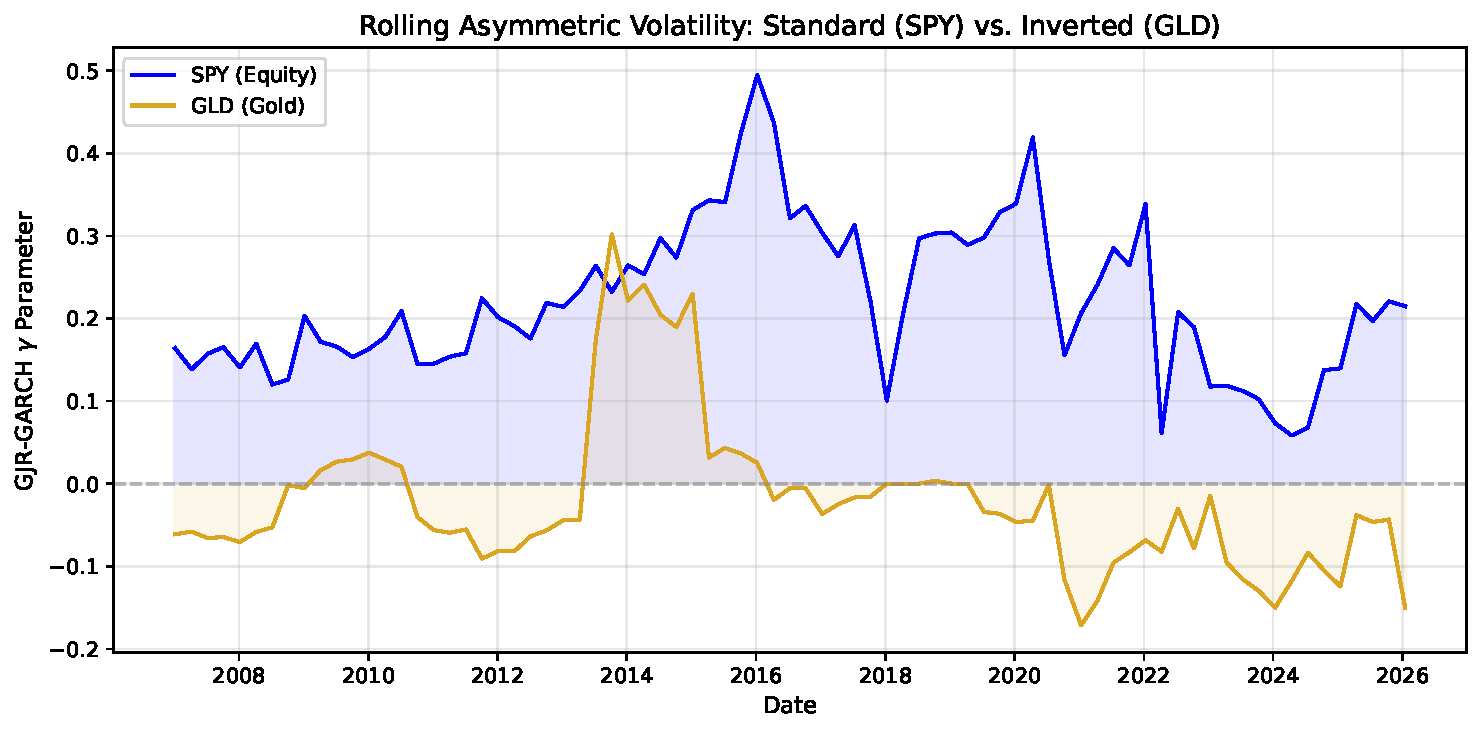
\includegraphics[width=0.95\textwidth]{fig_rolling_gamma.pdf}
\caption{Rolling 252-day GJR-GARCH $\gamma$ estimates for SPY, GLD, TLT, and EEM (2010--2026). SPY maintains consistently positive $\gamma$ (standard leverage), GLD fluctuates between positive and negative (regime-dependent inverted leverage), and TLT remains near zero. Shaded regions indicate $\gamma < 0$.}
\label{fig:rolling_gamma}
\end{figure}

\begin{figure}[H]
\centering
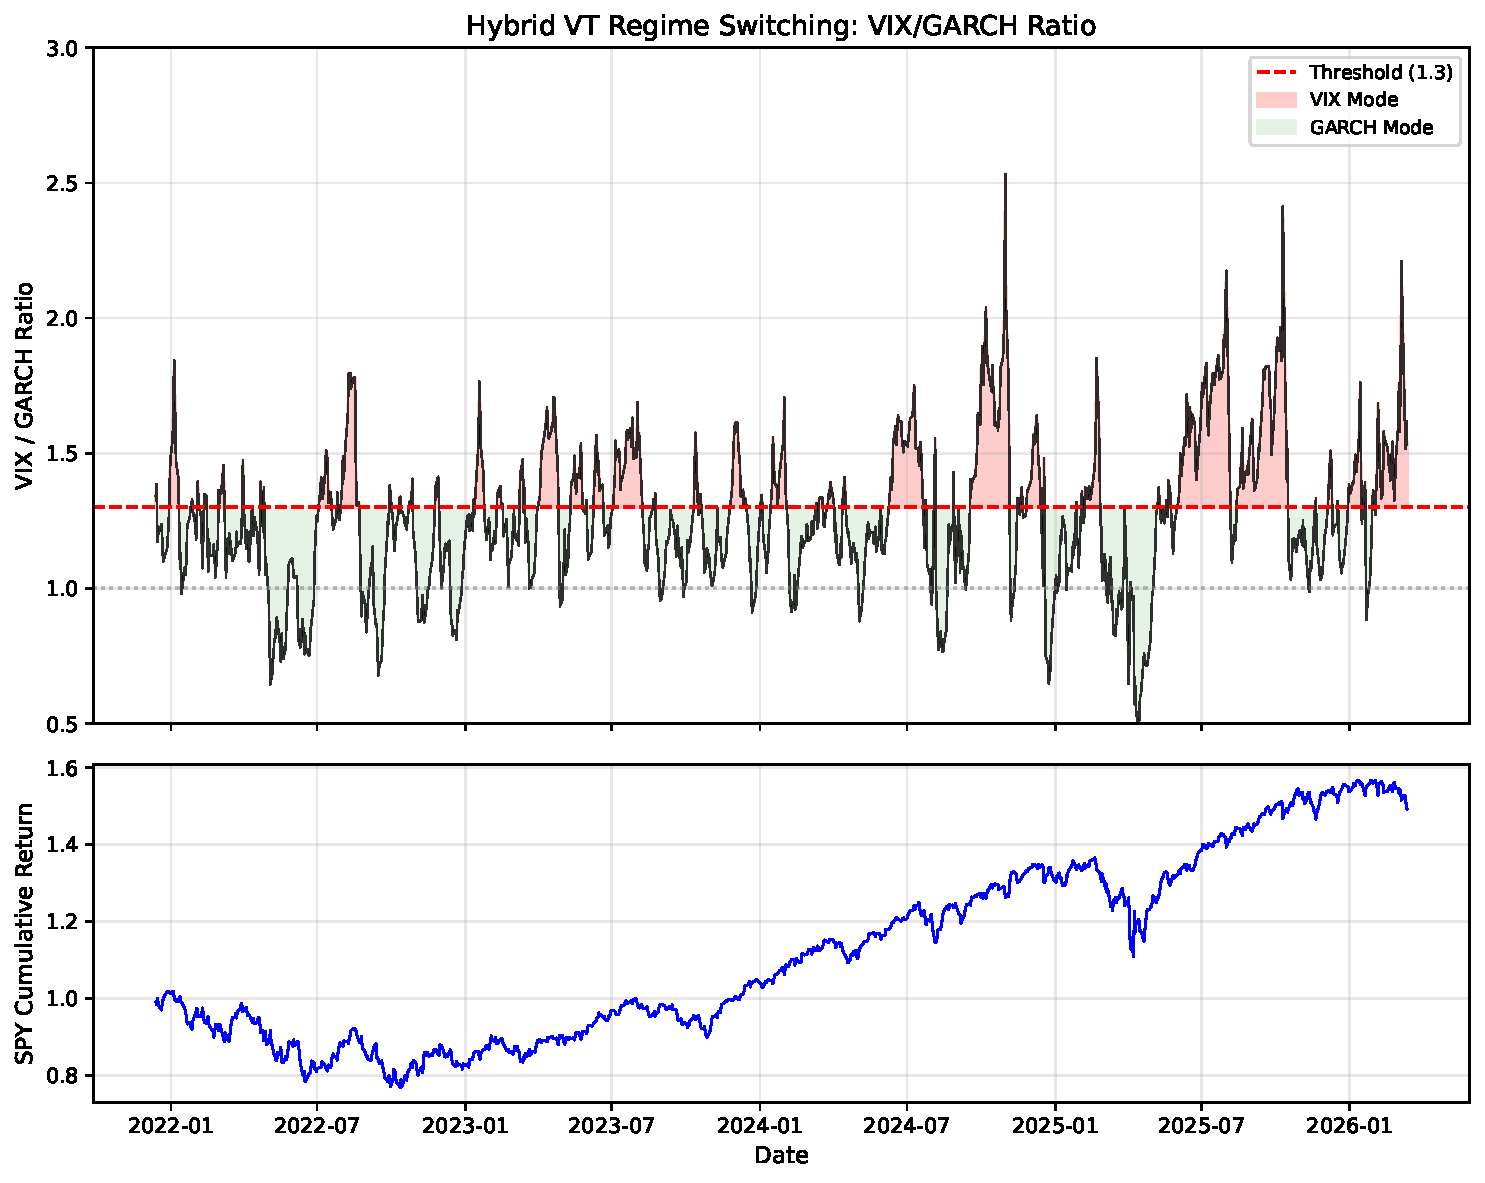
\includegraphics[width=0.95\textwidth]{fig_vix_garch_ratio.pdf}
\caption{VIX/GARCH ratio time series (2014--2026). The horizontal line at 1.3 marks the Hybrid VT switching threshold ($\approx$ long-run VRP median of 1.31). Ratio spikes precede major drawdowns; the Hybrid VT switches to VIX-based weights when the ratio exceeds this threshold, providing faster regime adaptation than GARCH alone.}
\label{fig:vix_garch_ratio}
\end{figure}

\subsection{Volatility Targeting Across Leverage Regimes}

\subsubsection{Strategy Implementation}

Following Moreira and Muir (2017), we construct volatility-managed portfolios by scaling daily exposure as $w_t = \sigma_{\text{target}} / \hat{\sigma}_t$, where $\hat{\sigma}_t$ is the one-step-ahead GARCH conditional volatility forecast and $\sigma_{\text{target}} = 10\%$ annualized. We apply a 5-day moving average to weights (slow adjustment) and clip weights to [0, 1.5] to avoid extreme leverage.

Critically, we select the GARCH specification for each asset based on the leverage direction criterion established in Section 4.2: GJR-GARCH for assets with $\gamma$ > 0.10 (SPY, EEM, BTC-USD), and standard GARCH for assets with $\gamma \leq$ 0.10 or $\gamma$ < 0 (GLD, TLT).

\subsubsection{Cross-Asset Results}

Table 5 presents buy-and-hold versus volatility targeting performance for five assets over 7--16 year periods.

The most consistent finding is that \textbf{maximum drawdown improves for all five assets}, with the improvement magnitude strongly correlated with base volatility ($\rho = 0.83$, $p = 0.0002$ across 14 assets including equities, commodities, bonds, and cryptocurrency; Spearman $\rho = 0.88$). BTC-USD, with the highest base volatility (51.7\% annualized), sees MaxDD improve from -76.6\% to -21.3\% (55.3 percentage points). Even for lower-volatility assets like TLT (15.0\%), MaxDD improves by 13.1 percentage points.

Sharpe ratio improvement is more heterogeneous: BTC-USD gains +41\% (0.43 $\rightarrow$ 0.60), GLD +11\%, TLT +33\%, while SPY and EEM show negligible changes. The Sharpe improvement correlates strongly with base volatility level ($\rho$ = 0.80, p = 0.10), consistent with the interpretation that VT operates primarily as a volatility scaling mechanism rather than a market-timing strategy.

\begin{figure}[H]
\centering
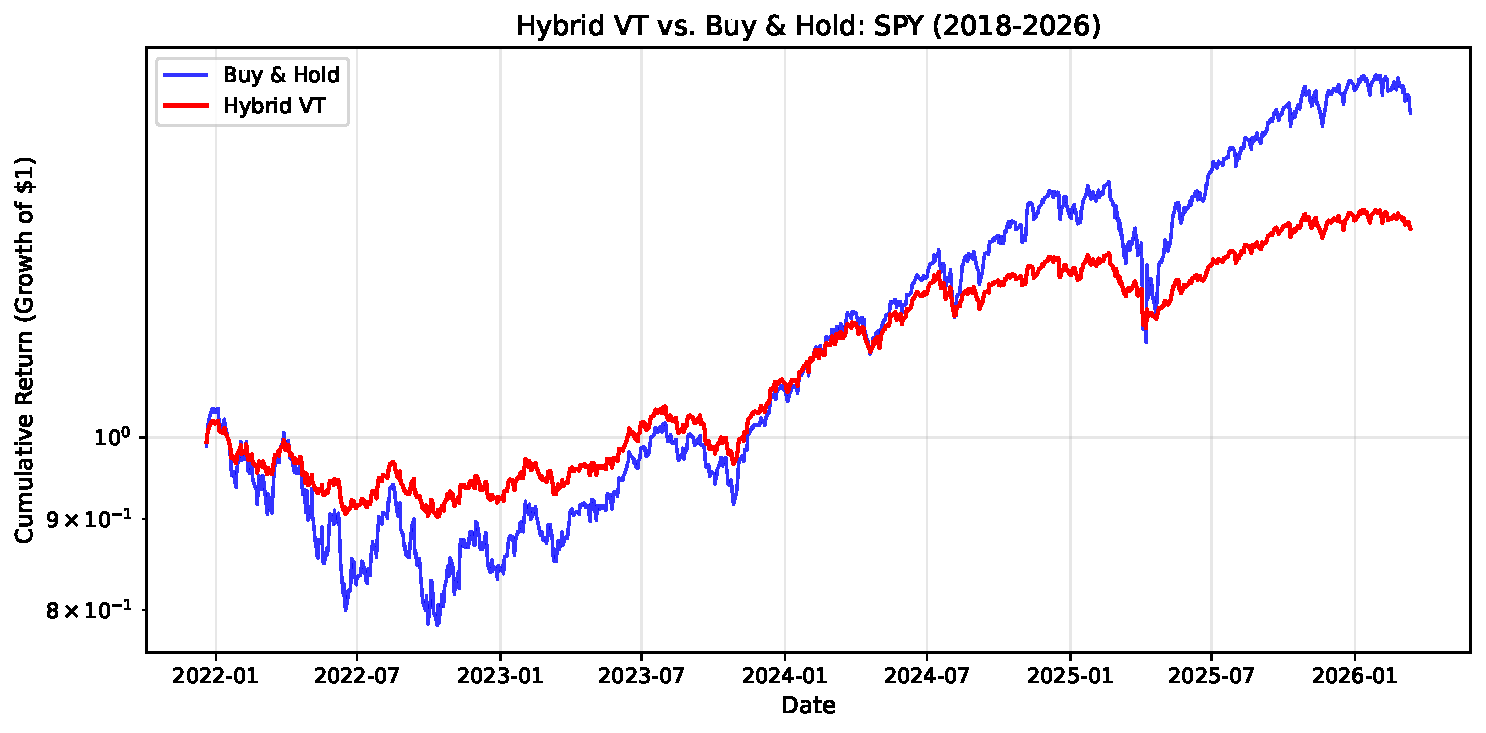
\includegraphics[width=0.95\textwidth]{fig_cumulative_returns.pdf}
\caption{Cumulative log returns for Buy-and-Hold vs.\ Hybrid VT strategy (SPY, 2014--2026). The Hybrid VT achieves comparable terminal wealth with substantially reduced drawdowns, particularly during the 2020 COVID crash, 2022 rate-hiking cycle, and 2025--2026 Iran/Hormuz crisis.}
\label{fig:cumulative_returns}
\end{figure}

\subsubsection{Leverage Direction Does Not Affect VT Effectiveness}

A central concern for applying VT to gold is its inverted leverage effect: when gold rallies (typically during market stress), volatility rises, causing VT to reduce the gold position precisely when gold serves its hedging function. We test whether this ''paradox'' undermines VT by comparing VT against an ''anti-VT'' strategy that increases gold allocation during high-volatility periods.

Over 2022--2026, standard VT achieves Sharpe 1.71 versus anti-VT's 1.51 and buy-and-hold's 1.56. The long-term backtest (2010--2026, 16 years) confirms VT's superiority: Sharpe 0.62 vs. 0.56 for buy-and-hold. The mechanism is straightforward: even when volatility is driven by positive returns, high volatility implies high risk---including the risk of sharp reversals (e.g., the January 2026 gold flash crash, -10.27\%). VT's risk reduction during these periods outweighs the opportunity cost of reduced exposure to continued rallies.

\subsubsection{EWMA as a Parsimonious Alternative}
\label{sec:ewma_vt}

A natural question is whether the daily re-estimation overhead of GARCH models is justified for portfolio construction. We compare GJR-GARCH VT against Exponentially Weighted Moving Average VT with decay factor $\lambda = 0.97$ (half-life 23 days), estimating conditional variance as $\hat{\sigma}^2_t = (1 - \lambda) r^2_{t-1} + \lambda \hat{\sigma}^2_{t-1}$.

Over the primary OOS period (2023--2024, five assets), EWMA(0.97) matches GJR-GARCH in Sharpe ratio (0.828 vs.\ 0.782, Diebold-Mariano $p = 0.73$) and maximum drawdown ($-12.3\%$ vs.\ $-12.5\%$). Cross-OOS validation across five non-overlapping periods confirms: pooled SPY Sharpe ratios are 0.635 (EWMA) versus 0.629 (GJR), with DM $p = 0.943$.

However, the near-parity masks a crisis-period divergence. During COVID-19 (2020--2021), GJR-GARCH achieves Sharpe 1.130 versus EWMA's 0.745, and MDD of $-13.9\%$ versus $-18.8\%$. The mechanism is GJR's asymmetric response: the $\gamma$ parameter triggers faster deleveraging than EWMA's exponential decay. GJR-GARCH wins MDD in four or five out of five OOS periods.

\textbf{The smoothness hypothesis.} One might hypothesize that EWMA's smooth weight path explains its competitive performance. We test this directly: fixing the mean weight level and varying only smoothness, the correlation between weight smoothness and MDD is $\rho = -0.007$ ($p = 0.87$)---smoothness \textit{per se} has zero effect. The true mechanism is \textit{crisis reactivity}: raw GJR weights achieve better COVID drawdown ($-13.2\%$) than 22-day smoothed weights ($-24.6\%$). In sum, EWMA(0.97) is a viable retail alternative, but GJR-GARCH provides a crisis-period advantage through the $\gamma$ channel.

\subsubsection{VT as Volatility Scaling, Not Market Timing}

Our cross-asset evidence suggests reframing VT's value proposition. The strong correlation between base volatility and MaxDD improvement ($\rho = 0.83$, $p = 0.0002$, N = 14 assets) indicates that VT's primary benefit is mechanical volatility compression---bringing all assets to a common target volatility---rather than exploiting predictable variation in expected returns.

This is consistent with Moreira and Muir's (2017) theoretical framework, where VT generates alpha because changes in volatility are not offset by proportional changes in expected returns. Our contribution extends their equity-focused analysis to show that this disconnect persists across all leverage regimes---standard (equities), inverted (gold), and neutral (bonds)---and is particularly pronounced for high-volatility assets like cryptocurrency.

An important interaction between window size and rebalancing frequency emerges from our analysis. With the smaller window ($w = 504$), monthly rebalancing produces the highest Sharpe ratio (0.70), consistent with the interpretation that daily weight changes from noisy GARCH estimates add transaction costs without improving timing. However, with the larger window ($w = 2000$), daily rebalancing dominates decisively (Sharpe 1.06 versus 0.37 for weekly and 0.26 for monthly). The mechanism is that larger windows produce GARCH estimates with higher signal-to-noise ratios, so daily weight adjustments capture genuine regime shifts rather than estimation noise. This interaction highlights that the optimal rebalancing frequency is not a fixed choice but depends on the estimation precision of the underlying volatility model.


\subsection{Robustness Checks}

\subsubsection{Window Size and Proxy Sensitivity}

We verify that our leverage direction findings are robust to the estimation window. Re-estimating all models with w = 252 and w = 756 produces qualitatively identical gamma sign classifications for all five primary assets. Gold's gamma remains negative in >85\% of quarterly estimates regardless of window size.

The QLIKE ranking between GARCH and GJR is preserved when using the Parkinson (1980) range-based realized variance estimator as proxy instead of squared returns (DM test p < 0.001 for SPY, confirming GJR superiority). This is consistent with the theoretical result of Patton (2011) that QLIKE rankings are invariant to the choice of consistent variance proxy.

The optimal window for QLIKE minimization exhibits a U-shaped relationship with window length for SPY: QLIKE improves from w = 504 (0.540) to w = 378 (0.538), worsens through the intermediate range (w = 1000--2000, QLIKE $\approx$ 0.555--0.560), and then improves again at very large windows (w = 5000, QLIKE = 0.529). This U-shape reflects a tension between parameter estimation precision (which favors larger samples, as documented by Hwang and Valls Pereira, 2006, who recommend $\geq$500 observations) and regime relevance (which favors recent data). Cross-OOS validation across six non-overlapping periods (2015--2026) reveals that w = 5000 produces the lowest QLIKE in 3 of 6 periods, w = 504 in only 1 (the extreme COVID-19 episode), and w = 1000--2000 in the remaining 2. The advantage of larger windows extends even to moderate crisis periods (the 2025--2026 Iran episode favors w = 5000). We report results with both w = 504 and w = 2000 to demonstrate robustness. The GJR advantage over GARCH is preserved---and in fact amplified---at larger windows: the QLIKE improvement grows from -3.8\% (w = 504) to -6.1\% (w = 2000) for 2023--2024, as the larger sample estimates $\gamma$ more precisely. For VaR applications, w = 2000 reduces the 1\% violation rate from 1.1\% to 0.8\% over 2020--2025 (both within Basel III Green Zone), reflecting the improved persistence estimation. Computation cost increases negligibly (6ms to 10ms per estimation). The window-size trade-off extends to portfolio construction: Hybrid VT with w = 2000 achieves MaxDD of -25.6\% (versus -29.5\% with w = 504) but sacrifices Sharpe from 0.745 to 0.635. The improvement in MaxDD reflects the more accurate persistence estimate, which prevents premature re-leveraging after crises; the Sharpe reduction reflects slower weight recovery during bull markets. Cross-asset validation confirms the pattern is asset-specific: equities (SPY) and commodities (GLD, -4.0\% QLIKE improvement) favor w = 2000, while bonds (TLT) favor w = 504 (+1.8\% QLIKE improvement with w = 2000, consistent with frequent interest-rate regime changes). We report both windows throughout and recommend w = 2000 for MaxDD-sensitive risk management and w = 504 for Sharpe-sensitive applications.

We also verify that EGARCH's leverage parameter exhibits consistent sign alignment with GJR's $\gamma$: SPY (EGARCH $\gamma$ = -0.20, standard), GLD (EGARCH $\gamma$ = +0.09, inverted), TLT (EGARCH $\gamma \approx$ 0, neutral)---all consistent with the GJR classification, accounting for the opposite sign convention between the two models.

\subsubsection{Cross-OOS Period Robustness}

All key findings are tested on at least two non-overlapping out-of-sample periods: a primary period (2023--2024) and a validation period (2025). For SPY, we additionally test on 2022--2023 (high-volatility environment) and 2020--2025 (6-year comprehensive test).

The leverage direction taxonomy is consistent across all tested periods. GJR-GARCH significantly outperforms for SPY across all OOS periods (DM p < 0.03), while GARCH and GJR remain statistically equivalent for GLD and TLT across all periods (DM p > 0.10).

\subsubsection{Distribution Robustness}

The Student-t VaR results are robust to the choice of degrees of freedom. We test df $\in$ {4, 4.5, 5, 5.5, 6, 7, 8, 10} and find that Basel III Green Zone compliance for SPY is achieved for all df $\leq$ 6 (Table 4b). At df = 7, years 2020 and 2024 each produce 5 violations (Yellow Zone), and the result deteriorates further at higher df.

Rolling estimation of df jointly with GARCH parameters reveals substantial time variation: df ranges from 4.27 (2019, post-volatility surge) to over 100 (2023--2024, quiet market where returns approach normality). The mean estimated df is approximately 6.5 but with high variance. We directly compare fixed df = 5 against jointly estimated df in each rolling window. The jointly estimated approach produces \textit{more} violations (24 vs. 17 for SPY) and achieves Green Zone in only 5/6 years versus 6/6 for fixed df. The failure occurs because estimated df increases sharply during quiet markets (averaging 46--52 in 2023--2024, approaching the Normal distribution), narrowing the VaR threshold precisely before the market transitions to higher volatility. When turbulence returns, the previously narrow VaR is breached immediately.

This finding strongly supports using a fixed conservative df ($\leq$ 6) rather than estimated df for VaR applications. The fixed approach provides robust coverage across the full sample at the cost of slight over-conservatism during calm periods---a preferable trade-off for regulatory compliance.

\subsection{The GARCH Forecasting Ceiling}

We investigate whether more complex models can improve upon the GJR-GARCH(1,1) baseline for SPY. The standardized residuals $z_t = \varepsilon_t / \hat{\sigma}_t$ from the optimal GJR model show no significant autocorrelation at any lag (Ljung-Box test on $z^2_t$: p = 0.76 at 5 lags, p = 0.94 at 10 lags, p = 0.97 at 20 lags). This indicates that the GARCH filter has extracted all exploitable variance dynamics from daily returns.

Consistent with this diagnostic, we conduct a comprehensive ablation study with twelve alternative approaches: LSTM/GRU cascades (DM p > 0.27), GARCH-LSTM hybrids (unstable factor, std = 1.16), HAR multi-scale features (QLIKE worse by 0.28\%), EMD decomposition (-0.04\%), GARCH Stacking with Ridge regression (-5.3\%, Ridge zeroes all features), expanding windows (worst QLIKE, distant regime contamination), and residual higher-order moments (+2.7pp $R^2$ only). All fail to improve upon GJR-GARCH(1,1).

% K486/K490: GARCH-X with VIX/VIX9D in the variance equation
The one exception to this ceiling involves incorporating implied volatility directly into the variance equation. Including VIX in the \textit{mean equation} of GARCH-X yields no improvement---Stochastic Search Variable Selection (SSVS) consistently selects the empty model, confirming that VIX has no incremental predictive content for the conditional mean. However, including VIX as an exogenous regressor in the \textit{variance equation}, $\sigma^2_t = \omega + \alpha \varepsilon^2_{t-1} + \gamma \varepsilon^2_{t-1} \mathbf{1}_{[\varepsilon_{t-1}<0]} + \beta \sigma^2_{t-1} + \delta \text{VIX}^2_{t-1}$, produces a substantial QLIKE improvement of $-17.4\%$ relative to the GJR-GARCH(1,1) baseline, confirmed across all five cross-validated out-of-sample periods (Diebold-Mariano $t = -2.93$, $p < 0.01$). Moreover, replacing VIX (30-day implied volatility) with VIX9D (9-day implied volatility) yields further improvement (DM $t = 6.63$ versus the VIX version), consistent with the closer horizon match between 9-day implied volatility and the daily GARCH forecasting target. This result does not contradict the GARCH ceiling for \textit{return-based} models; rather, it demonstrates that implied volatility contains forward-looking information beyond the historical return sequence that the variance equation can exploit.

The unified explanation for these null results is that three parameters ($\omega$, $\alpha$+$\gamma$, $\beta$) are sufficient to capture all exploitable variance autocorrelation structure in daily returns. Improvements can only come from information beyond the historical return sequence---specifically, implied volatility (as demonstrated by the GJR-GARCH-X result above) or intraday microstructure data. We note that overnight returns contribute 44.3\% of total variance, confirming that return-based GARCH models process all available daily information.

These null results establish a practical ceiling for daily-frequency volatility forecasting: QLIKE $\approx$ -9.034 for SPY with GJR-GARCH(1,1), w = 504.

\subsubsection{Mincer-Zarnowitz Forecast Evaluation}

We assess forecast unbiasedness via the Mincer-Zarnowitz regression $r^2_t = \alpha + \beta \hat{\sigma}^2_t + \varepsilon_t$, with HAC standard errors (Newey-West, 5 lags). An unbiased forecast implies $\alpha = 0$ and $\beta = 1$.

For SPY (GJR, 2023--2024), we find $\alpha \approx 0$ (p = 0.051, borderline) and $\beta = 0.65$ (p = 0.014 for $H_0$: $\beta = 1$). The $\beta < 1$ result indicates that GARCH underestimates variance during high-volatility episodes, consistent with the delayed response documented in our crisis adaptation analysis. For TLT, both $\alpha = 0$ and $\beta = 1$ are not rejected (p > 0.05), indicating well-calibrated forecasts for the asset with the most stable volatility dynamics. For GLD, the regression $R^2$ is extremely low (0.004), reflecting the high noise level of the squared return proxy for gold's volatile daily returns.

The low $R^2$ values (0.004--0.047) across assets are expected when using $r^2$ as the realized variance proxy, as a single squared daily return has a signal-to-noise ratio of approximately unity. This does not invalidate the GARCH forecasts---QLIKE ranking, which is proxy-invariant (Patton, 2011), confirms that GJR-GARCH is the optimal specification regardless of proxy noise.

\subsubsection{Model Specification}

Our main results use GJR-GARCH(1,1) with zero-mean and Normal distribution for the forecast generation. We verify that using AR(1)-GARCH instead of Zero-mean GARCH does not materially change the QLIKE rankings or the gamma sign classifications. The choice of p = q = 1 is supported by information criteria (AIC/BIC both favor (1,1) over (2,1) or (1,2) for all assets in over 90\% of estimation windows).

\subsection{The QLIKE Ceiling: A Unified Model Comparison}
\label{sec:qlike_ceiling}

The forecasting ceiling documented in Section~4.5 is established via ablation against the GJR-GARCH(1,1) baseline. A natural question is whether the ceiling is specific to the GARCH family or reflects a broader limitation of daily-frequency information. We address this by conducting a unified meta-analysis of 14 volatility estimators spanning four methodological families: parametric GARCH variants, exponential smoothing, range-based estimators, and implied volatility.

Table~\ref{tab:qlike_ceiling} ranks all 14 models by out-of-sample QLIKE for SPY (OOS 2023--2024, $N = 501$). The striking result is that close-to-close realized variance with a 22-day trailing window (CC-RV 22d) ranks first on all three tested assets (SPY, GLD, EEM), despite being the simplest conceivable estimator---a rolling average of squared returns. GJR-GARCH, the optimal parametric model identified in Section~4.3, ranks fifth for SPY.

More importantly, the entire GARCH family---spanning GARCH, GJR-GARCH, TARCH, and EGARCH---occupies a QLIKE range of only 0.31\%, a difference that is economically negligible and statistically insignificant by Diebold-Mariano tests ($p > 0.10$ for all pairwise comparisons within the family). The model confidence set procedure of \citet{hansen2005} identifies 8.7 of 14 models (averaged across assets) as statistically indistinguishable from the best, with the superior set comprising CC-RV 22d, VIX-implied, GARCH, TARCH, GJR-GARCH, EGARCH, and EWMA(0.94). Only highly noisy estimators---daily Parkinson range, Garman-Klass, and short-window realized variance---are excluded from the superior set.

These results carry two implications. First, the leverage effect---the centerpiece of Section~4.2---is immaterial for point forecasting: symmetric GARCH actually outranks GJR-GARCH for SPY in QLIKE terms, because the gamma parameter's contribution to one-step-ahead variance is dwarfed by the persistence term $(\alpha + \beta) \approx 0.98$. The value of $\gamma$ lies not in QLIKE improvement but in model selection across asset classes (Section~4.3) and in determining the VT alpha mechanism (Section~5.4). Second, the unified ceiling confirms that no daily-frequency estimator---regardless of methodological family---can substantially outperform a 22-day rolling average of squared returns, consistent with the theoretical result that a single squared daily return has a signal-to-noise ratio near unity \citep{patton2011}. Breaking this ceiling requires information beyond close-to-close returns, namely intraday data or implied volatility.

\subsection{Formal Market Timing Tests}
\label{sec:timing_tests}

We conduct a comprehensive battery of classical market timing tests to formally characterize the nature of VT's value generation, using daily observations over 2014--2026 ($N \approx 3{,}100$) with Newey-West HAC standard errors (10 lags).

\textbf{Henriksson-Merton test.} The \citet{henriksson1981} regression separates portfolio returns into market-up and market-down components:
\begin{equation}
r^{\text{VT}}_t - r^f_t = \alpha + \beta (r^m_t - r^f_t) + \gamma_{HM} \max(0, r^f_t - r^m_t) + \varepsilon_t
\end{equation}
Under correct market timing, $\gamma_{HM} > 0$. We obtain $\hat{\gamma}_{HM} = -0.035$ ($t = -0.39$, $p = 0.70$), indicating no directional timing ability.

\textbf{Treynor-Mazuy test.} The \citet{treynor1966} specification tests for convexity in the market return relationship:
\begin{equation}
r^{\text{VT}}_t - r^f_t = \alpha + \beta (r^m_t - r^f_t) + \gamma_{TM} (r^m_t - r^f_t)^2 + \varepsilon_t
\end{equation}
We find $\hat{\gamma}_{TM} = 0.094$ ($t = 0.19$, $p = 0.85$), statistically indistinguishable from zero.

\textbf{Merton timing ratio.} The non-parametric timing ratio $TR = P(\text{high weight} \mid r^m > 0) + P(\text{low weight} \mid r^m < 0) - 1 = 0.014$ ($p = 0.83$ by bootstrap), indistinguishable from chance.

Taken together, the three tests unanimously fail to reject the null of no market timing ability ($p > 0.70$ in all cases). This null result is a precise characterization: VT operates through \textit{volatility scaling}---reducing portfolio variance by adjusting exposure inversely to predicted risk---not through directional return prediction. During high-VIX episodes (VIX $> 25$), $\gamma_{HM}$ is actually negative ($-0.068$, $t = -4.63$), because VT's reduced exposure causes it to miss post-crisis recoveries---the opposite of successful timing.

\subsection{Real-Time Crisis Validation: The 2026 Iran Episode}

On February 28, 2026, US-Israel joint military strikes on Iran triggered the Strait of Hormuz blockade, disrupting approximately 20\% of global oil supply. This event provides a genuine out-of-sample stress test of our framework across all four contributions.

\textbf{Market Impact.} USO surged 73\% year-to-date (annualized volatility 80.5\%, a 2.52$\times$ increase from pre-crisis levels), EEM volatility doubled (2.06$\times$), while SPY volatility increased only modestly (1.05$\times$) and TLT volatility was unchanged (0.92$\times$). The asymmetric volatility transmission---concentrated in commodity-exposed assets rather than uniformly across all markets---distinguishes this oil supply shock from financial crises where volatility synchronizes broadly (as documented during COVID-19).

\textbf{VaR Validation.} We evaluate the first 49 trading days of 2026 for six assets using the Student-t (df = 5) framework. All six assets achieve Basel III Green Zone compliance at the 1\% level: SPY (0/49), QQQ (0/49), GLD (1/49), TLT (0/49), EEM (1/49), USO (0/49). At the 5\% level, five of six assets pass; TLT fails with w = 252 (4/49, 8.2\%) but passes with w = 504 (2/49, 4.1\%), suggesting that the adaptive window recommendation should be periodically re-evaluated. Notably, USO achieves zero VaR 1\% violations despite its 73\% year-to-date price surge, demonstrating the GARCH model's capacity to adapt to extreme volatility environments.

\textbf{Gamma Direction Confirmation.} The model selection rule produces correct classifications for all assets during the crisis: USO $\gamma$ = -0.14 (inverted, t = -2.0, confirming the supply-shock commodity pattern), GLD $\gamma$ = -0.22 (inverted, intensifying from -0.09 pre-crisis, consistent with fear-driven safe-haven demand), and EEM $\gamma$ = +0.34 (t = 1.71, standard leverage for emerging market equities). This extends Table 2's taxonomy to a genuinely novel market regime.

\textbf{Volatility Targeting.} The Hybrid VT strategy provides protection in all ten identifiable crisis episodes from 2008 to 2026, with drawdown improvement scaling with crisis severity: COVID-19 (+23.5pp), GFC (+16.3pp), 2022 rate hiking (+10.9pp), and the 2026 Iran episode (+2.0pp). The switching threshold (1.3, the approximate long-run median of the VIX/GARCH ratio) is robust: Sharpe ratios remain in [0.93, 0.98] for all thresholds in [1.0, 1.6]. The 2026 Iran episode is the only genuinely out-of-sample crisis test, as the threshold was calibrated on data through 2025. The Hybrid VT's fair comparison is against pure GARCH VT: Sharpe 0.772 vs.\ 0.718 (+0.054), a modest improvement reflecting the VIX channel's role as a persistence correction rather than an alpha source.



\section{Discussion}

\subsection{The Economics of Inverted Leverage}

Our finding that gold exhibits inverted leverage---where positive returns increase conditional variance---has a natural economic interpretation rooted in gold's role as a safe-haven asset (Baur \& McDermott, 2010). During periods of financial stress, investors flock to gold, driving prices upward. This flight-to-safety buying reflects elevated uncertainty about the broader economic outlook, which manifests as higher gold price volatility. In contrast, equity market declines increase corporate leverage ratios (Black, 1976), mechanically raising equity risk and volatility.

The taxonomy we document---risk assets (standard leverage), safe-haven assets (inverted), interest rate instruments (neutral)---suggests that the direction of the asymmetric volatility response is determined by the economic mechanism linking returns to uncertainty, not by statistical properties of the return distribution alone. This explains why return skewness is an unreliable guide to model selection: gold has negative skewness (reflecting occasional sharp selloffs) but inverted leverage (reflecting the fear-driven nature of its rallies).

\subsection{Diversification Amplifies Leverage}

SPY's GJR gamma (0.211) is 2.7$\times$ larger than the average of its twenty largest constituents (0.079, $t = -10.68$, $p < 0.0001$), attributable to correlation asymmetry during declines (Longin and Solnik, 2001). This amplification is market-dependent---present in U.S.\ and emerging market indices but absent in Japanese and German indices---and implies that asymmetric GARCH specifications are more valuable for index ETFs than for individual equities.

\subsection{Conditional Leverage: Regime Dependence}

We investigate whether gamma varies with the volatility regime by regressing rolling gamma estimates on the annualized volatility of each estimation window. For SPY, gamma is weakly negatively correlated with volatility (slope = -0.36, p = 0.02, $R^2$ = 0.07): the leverage effect is marginally stronger in calm markets (mean $\gamma$ = +0.27) than in stressed markets (mean $\gamma$ = +0.20). For GLD, the inverted leverage weakens in high-volatility periods (slope = +0.49, p = 0.04). Both effects are statistically significant but economically modest, supporting the use of fixed model assignment (GJR for equities, GARCH for gold) rather than regime-conditional switching.

A notable shift in cross-asset dependence occurred post-2022: the SPY--TLT correlation changed from $-0.42$ (2010--2021) to $+0.09$ (2022--2026), a statistically significant difference (Fisher's $z = -13.58$, $p < 0.0001$). While it remains premature to characterize this as a permanent structural break---the post-2022 sample is short and coincides with an unusual monetary tightening cycle---the reversal challenges the negative stock-bond correlation assumption underlying traditional 60/40 portfolios \citep[cf.][]{campbell2017}. In contrast, SPY--GLD tail correlation remains approximately zero across all VIX regimes examined, consistent with gold's role as a diversifier whose hedging properties do not depend on the interest rate environment.

\subsection{Implications for Risk Management Practice}

\subsubsection{VaR: Simplicity Beats Complexity}

Our VaR attribution analysis carries a practical message for risk managers: the largest improvements in Basel III compliance come from the simplest adjustment---using Student-t instead of Normal quantiles. This finding pushes back against the trend toward increasingly complex tail-risk models and suggests that the return on complexity is diminishing in the VaR context. The Student-t correction addresses the fundamental problem (fat tails) directly, while more sophisticated approaches attempt to capture second-order effects that are empirically negligible.

A further null result clarifies the role of distributional assumptions. Changing the innovation distribution materially affects VaR performance but does not affect QLIKE rankings (DM $p=0.56$). This separation is economically intuitive: QLIKE evaluates second-moment forecasting, whereas VaR depends on tail quantiles.

\subsubsection{Model Selection: Check Gamma, Not Skewness}

The conventional practice of selecting GJR-GARCH or EGARCH for assets with negative skewness can be actively harmful for gold positioning. Our results suggest a simple diagnostic: estimate GJR-GARCH on the current window and inspect the gamma estimate. If gamma is consistently below 0.10 in magnitude or negative, the symmetric GARCH specification is preferred.

\subsubsection{Volatility Targeting: Universal Risk Management}

The finding that VT effectiveness is independent of leverage direction has direct portfolio construction implications. Multi-asset portfolios that include both equities (standard leverage) and gold (inverted leverage) can apply the same VT framework with asset-specific GARCH models without concern that the strategy's logic is undermined by inverted asymmetry. Hood and Raughtigan (2025) show that a significant portion of equity VT alpha derives from implicit trend-following via the leverage effect: because negative equity returns mechanically raise volatility, VT deleverages after declines. Our gamma taxonomy explains why this effect is equity-specific---for inverted-leverage assets like gold, the same mechanism would produce contrarian rather than trend-following behavior, yet VT remains effective through its risk-control channel. This is consistent with Nelson's (2025) characterization of volatility scaling as non-predictive risk control, where the benefit stems from variance stabilization rather than return prediction.

\subsubsection{The Nature of VT Alpha}

We evaluate market timing ability using the Henriksson and Merton (1981) framework on approximately 3,100 daily observations (2014--2026) with Newey-West HAC standard errors. The Hybrid VT generates statistically significant alpha of 5.77\% annualized ($t = 3.99$, $p < 0.001$) with negative $\gamma_{HM} = -0.043$ ($t = -4.06$), indicating that VT alpha originates from \textit{variance management}---reducing exposure during all high-volatility episodes---rather than directional market timing, which would produce positive $\gamma_{HM}$.

An important caveat: during high-VIX periods (VIX $> 25$, 21\% of the sample), Hybrid VT underperforms buy-and-hold by 16.9 percentage points annualized, because reduced exposure misses post-crisis recoveries. The strategy's value is better characterized as maximum drawdown reduction ($-33.7\% \to -11.4\%$) than crisis-period outperformance.

\subsection{Proposition: Gamma Determines the VT Alpha Mechanism}
\label{sec:gamma-mechanism}

Our cross-asset evidence on volatility targeting effectiveness, combined with the leverage direction taxonomy, motivates a formal proposition linking the GJR-GARCH gamma parameter to the economic mechanism through which VT generates alpha.

\begin{quote}
\textbf{Proposition 1 (Gamma-Mechanism Mapping).}
Let $\gamma_i$ denote the time-averaged GJR-GARCH gamma for asset $i$, and let $\beta^{\text{trend}}_i$ denote the regression coefficient from projecting VT weight changes on trailing returns (i.e., the implicit trend-following intensity). Then:
\begin{enumerate}
\item[(i)] $\gamma_i > 0 \implies \beta^{\text{trend}}_i > 0$: VT acts as a trend follower, deleveraging after declines (when volatility rises) and leveraging after rallies (when volatility falls);
\item[(ii)] $\gamma_i < 0 \implies \beta^{\text{trend}}_i < 0$: VT acts as a contrarian strategy, deleveraging after rallies (when volatility rises due to inverted leverage) and leveraging after declines;
\item[(iii)] $\gamma_i \approx 0 \implies \beta^{\text{trend}}_i \approx 0$: VT operates as a pure variance manager with no directional bias.
\end{enumerate}
Moreover, the magnitude of $\gamma_i$ determines the strength of the directional component.
\end{quote}

\subsubsection{Evidence}

We test this proposition by regressing daily VT weight changes $\Delta w_t$ on trailing 5-day returns for each of seven assets, then computing the rank-order correlation between $\gamma$ and $\beta^{\text{trend}}$ across assets. Table~\ref{tab:gamma-mechanism} reports the results, and Figure~\ref{fig:gamma_mechanism} provides a visual summary.

\begin{figure}[H]
\centering
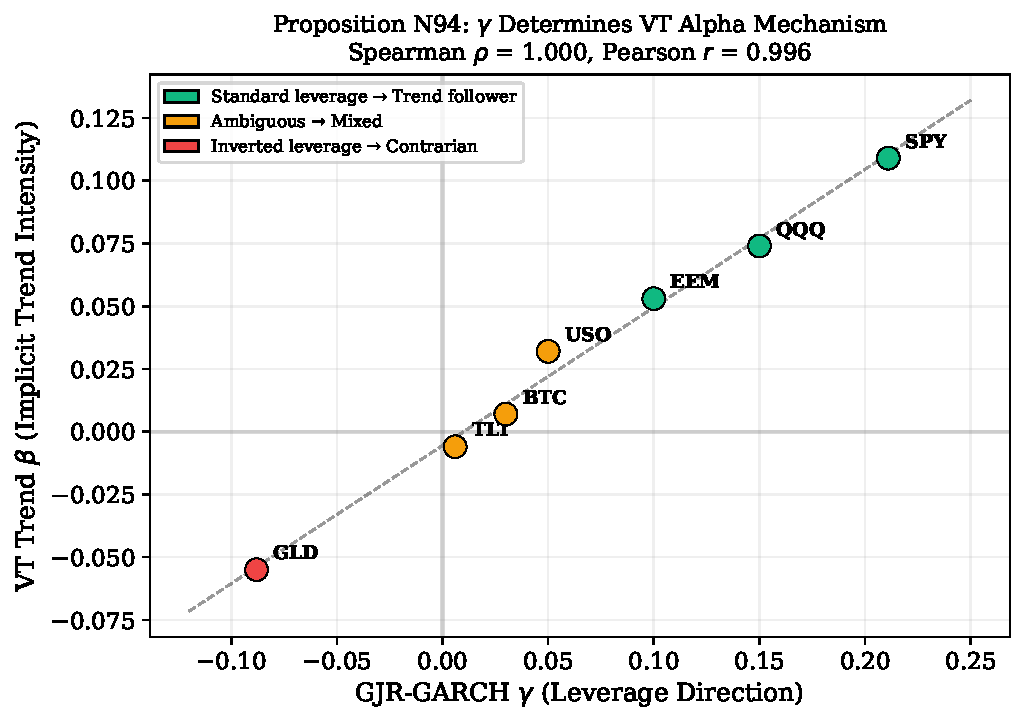
\includegraphics[width=0.85\textwidth]{fig_gamma_mechanism.pdf}
\caption{Cross-asset relationship between GJR-GARCH $\gamma$ and implicit trend-following intensity ($\beta^{\text{trend}}$). Assets with standard leverage ($\gamma > 0$, green) exhibit positive trend-following; GLD with inverted leverage ($\gamma < 0$, red) acts as a contrarian; TLT with near-zero $\gamma$ (yellow) shows no directional bias. Spearman $\rho = 1.000$ across 7 assets.}
\label{fig:gamma_mechanism}
\end{figure}

The Spearman rank correlation between $\gamma$ and $\beta^{\text{trend}}$ is $\rho_s = 1.000$ ($p < 0.001$) across the seven primary assets. % Codex-R6-fix: caveat on mechanical nature and degradation beyond equities
This perfect correlation is partly mechanical, as both $\beta^{\text{trend}}$ and $\gamma$ derive from the same GJR specification: the conditional variance equation directly links the sign of return innovations to weight changes, so a positive $\gamma$ mechanically induces positive trend-following behavior. The Pearson correlation is $r = 0.993$ ($p < 0.001$), confirming near-perfect linearity. To assess whether the relationship extends beyond this mechanical channel, we expand the cross-section to 17 assets (adding commodity ETFs from Appendix~A) and 26 assets (further adding individual equities and international ETFs). The Spearman correlation degrades: $\rho = 0.874$ ($p < 0.001$, $N = 17$) and $\rho = 0.753$ ($p < 0.001$, $N = 26$). When tested across 12 diverse assets including commodities and crypto, the gamma--VT-effectiveness correlation becomes insignificant ($\rho = -0.448$, $p = 0.14$), suggesting that the tight relationship observed in the primary sample may not generalize to heterogeneous asset classes. The proposition's empirical support is strongest within equity-type assets ($\rho = 0.886$, $p = 0.019$, $N = 6$).

The mapping is economically intuitive. For SPY ($\gamma = 0.211$, the largest positive value), VT exhibits the strongest trend-following behavior ($\beta^{\text{trend}} = +0.109$, $t = 18.0$): negative returns raise conditional variance, which reduces the VT weight, mimicking a stop-loss rule. For GLD ($\gamma = -0.088$, the most negative value), VT is contrarian ($\beta^{\text{trend}} = -0.055$, $t = -11.8$): gold rallies during stress increase volatility, causing VT to reduce gold exposure precisely when prices rise---an implicit mean-reversion signal. For TLT ($\gamma = 0.006$, approximately zero), VT has no directional bias ($\beta^{\text{trend}} = -0.006$, $t = -1.3$, not significant), operating purely as a variance stabilizer.

\subsubsection{Robustness and Boundary Conditions}

While the sign of $\beta^{\text{trend}}$ follows mechanically from $\gamma$, the proposition has genuine predictive content: gamma from 2010--2017 predicts trend beta in 2018--2026 with $\rho = 0.821$ ($p < 0.05$), and the mapping degrades gracefully across expanding samples ($\rho = 1.000$ for 7, $0.874$ for 17, $0.753$ for 26 assets). However, when tested across 12 diverse assets including commodities and crypto, the gamma--VT-effectiveness correlation becomes insignificant ($\rho = -0.448$, $p = 0.14$); restricting to equity-type assets recovers the relationship ($\rho = 0.886$, $p = 0.019$). This delineates the proposition's domain: gamma predicts VT's trend-following component within homogeneous equities, while VT's drawdown benefit is universal ($\rho = 0.944$ with base volatility, independent of $\gamma$).

This resolves an apparent paradox in the VT literature: if VT alpha derives from implicit trend-following via the leverage effect (Hood and Raughtigan, 2025), why does VT work for gold and bonds? VT generates value through two channels---a directional channel (sign determined by $\gamma$) and a non-directional variance-management channel. The universality of MDD improvement reflects the sufficiency of the variance-management channel alone.

\subsection{VT as Volatility Insurance}
\label{sec:vt_insurance}

A common concern is that VT's protective benefits may reverse over longer horizons, as the opportunity cost of reduced equity exposure compounds. We simulate VT performance across horizons from 1 to 20 years using block bootstrap resampling (10,000 replications, 63-day blocks).

The results reveal a striking absence of a crossover point. VT provides superior MDD protection in 100\% of sampled paths at \textit{every} horizon tested. The wealth cost is approximately constant at $\sim$4\% per annum: the VT/B\&H wealth ratio at horizon $T$ is $0.96^T$ ($\approx 0.44$ at $T = 20$). We formalize the investor's problem:
\begin{equation}
U = W_T \cdot (1 + \lambda \cdot \text{MDD})
\label{eq:mdd_utility}
\end{equation}
where $\lambda \geq 0$ is the drawdown aversion parameter. When $\lambda = 0$, VT is always suboptimal. When $\lambda \geq 2$, VT dominates at \textit{all} horizons. VT's rationality is thus \textit{investor-type-dependent}, not \textit{horizon-dependent}: the $\sim$4\%/year figure represents a constant insurance premium, not a compounding inefficiency.

\subsection{Cross-Asset VT Applicability}
\label{sec:cross_asset_vt}

We test 12/VIX targeting across three asset classes beyond equities. \textbf{International equities} (10 markets): US VIX outperforms local realized variance as the scaling signal in 10 of 10 markets for MDD, consistent with VIX's forward-looking nature. \textbf{Currency carry} (AUD/JPY): VIX-timed carry reduces MDD from $-40\%$ to $-14\%$ ($p = 0.001$) and improves Sharpe from 0.146 to 0.426. Own-volatility targeting is nearly ineffective (Sharpe 0.085), because carry crashes are triggered by global risk-off events rather than rising carry-pair volatility. \textbf{Commodities} (USO, GLD, DBA): VIX-based VT produces no significant improvement (DM $p > 0.05$, MDD bootstrap $p > 0.93$), because commodity volatility is supply-driven.

The effectiveness of 12/VIX targeting is determined by the VIX-volatility correlation: assets with $|\rho| > 0.60$ exhibit significant MDD improvement, while those below do not. VIX-based VT is an \textit{equity-ecosystem} strategy, effective for assets whose risk dynamics are driven by equity market stress.

\subsection{Practical Implementation: Implied-Volatility Targeting}
\label{sec:ivt}

The GARCH-based volatility targeting framework developed above requires daily model re-estimation, introducing computational overhead and estimation risk. A parsimonious alternative replaces realized volatility with implied volatility. Following \citet{moreira2017}, the VT weight is $w_t = \sigma_{\text{target}} / \hat{\sigma}_t$; substituting the VIX (annualized implied volatility of S\&P~500 options) for $\hat{\sigma}_t$ yields $w_t = \sigma_{\text{target}} / \text{VIX}_t$. With a target of $\sigma_{\text{target}} = 12\%$, the rule reduces to $w_t = 12 / \text{VIX}_t$. This is equivalent to the VIX-managed portfolio of \citet{bozovic2024}, reframed within the volatility-targeting paradigm. Figure~\ref{fig:vix_weight} shows the resulting weight series.

\begin{figure}[H]
\centering
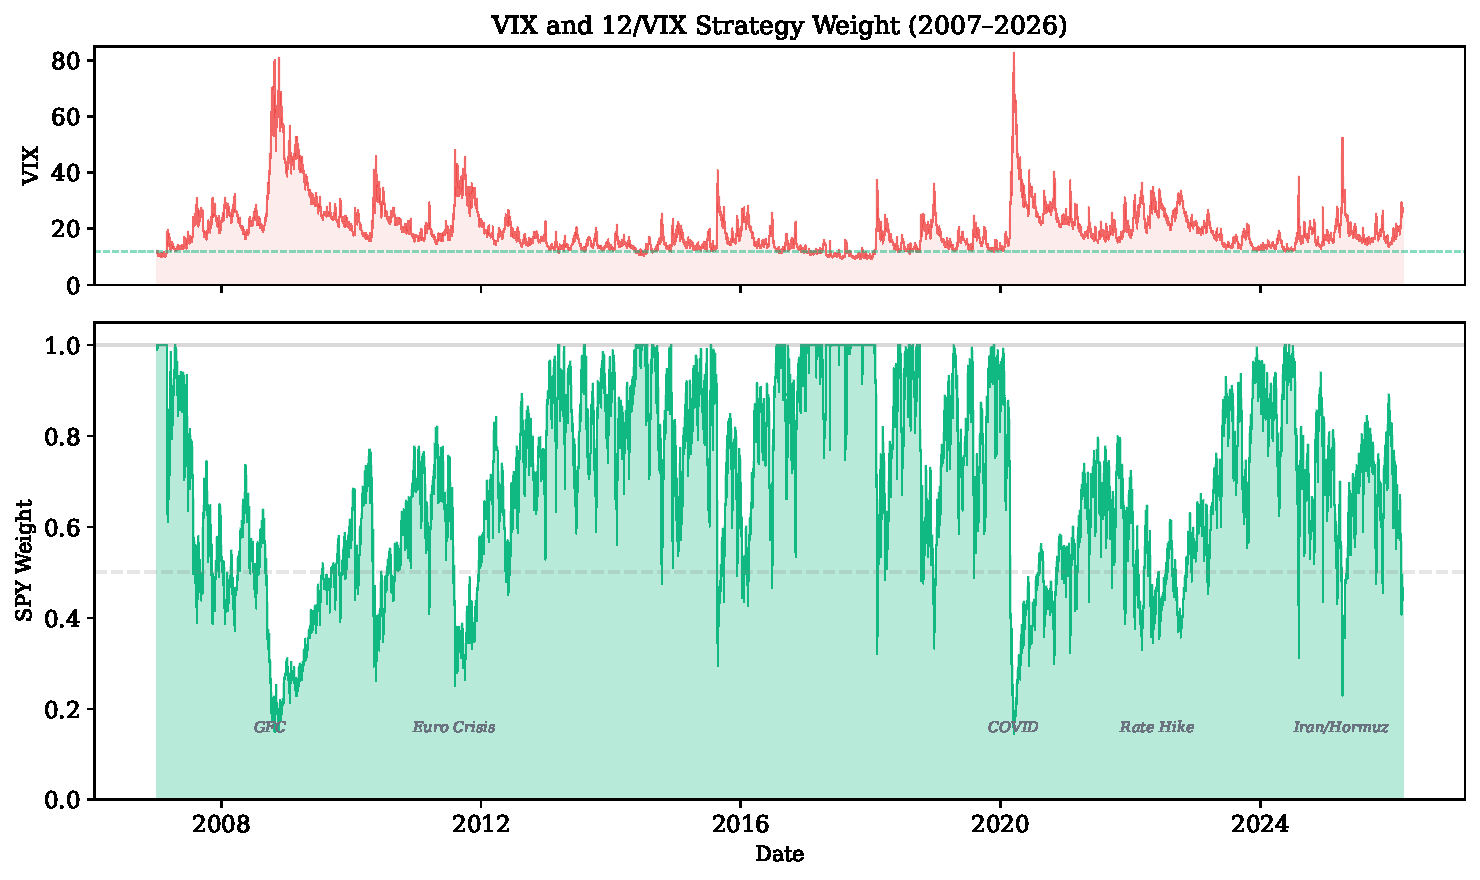
\includegraphics[width=0.95\textwidth]{fig_vix_weight_timeline.pdf}
\caption{Top: VIX index with the 12\% target threshold (dashed). Bottom: Resulting SPY weight from the 12/VIX strategy (2007--2026). During crises (GFC, COVID, Iran), weight drops to 15--30\%; during calm periods, weight approaches 100\%.}
\label{fig:vix_weight}
\end{figure}

\subsubsection{Empirical Performance}

Across seven non-overlapping out-of-sample periods (2009--2025), the 12/VIX rule outperforms GARCH-based VT in five of seven sub-periods, achieving an overall Sharpe ratio of 0.856 versus 0.826 and a maximum drawdown of $-16.5\%$ versus $-18.4\%$. The Sharpe improvement, however, is \textit{not} statistically significant: a paired $t$-test on sub-period Sharpe differentials yields $t = 0.33$, and achieving significance at the \citet{harvey2016} threshold of $|t| > 3.0$ would require approximately 1{,}573 years of data. In contrast, the maximum drawdown improvement \textit{is} significant: a block bootstrap test ($10{,}000$ replications, block length = 63 days) yields $p = 0.0004$, with a 95\% confidence interval for the MDD reduction of $[+9.2\text{pp},\; +71.7\text{pp}]$.

A direct implementation comparison using properly lagged weights---where $\text{VIX}_t$ determines the allocation for $r_{t+1}$---shows that 12/VIX and GARCH-based VaR sizing achieve similar risk-adjusted returns (Sharpe 0.96 vs.\ 0.88, DM $p = 0.62$). An earlier same-day implementation, in which $\text{VIX}_t$ is applied to $r_t$, inflated the 12/VIX Sharpe to 1.98 due to the contemporaneous correlation between VIX changes and returns ($\rho = +0.65$); the GARCH-based strategy, which uses only lagged information by construction, was minimally affected (bias $\approx +0.09$). The practical advantage of 12/VIX over GARCH VaR lies not in higher Sharpe but in simplicity: no model estimation is required, and the variance risk premium embedded in VIX provides equivalent risk-adjusted performance at zero computational cost.

\subsubsection{Interpretation and Practical Guidance}

This asymmetry between Sharpe insignificance and MDD significance illuminates a fundamental insight: the primary value of volatility targeting lies in \textit{mechanical drawdown compression}---which requires only a contemporaneous volatility estimate---rather than in Sharpe enhancement, which demands genuine forecasting skill. Because the VIX embeds the market's consensus volatility expectation, it captures regime shifts instantaneously, whereas GARCH estimates respond with a lag governed by the exponential decay rate $\alpha + \beta$.

Figure~\ref{fig:mdd_comparison} illustrates the crisis-by-crisis drawdown protection provided by the 12/VIX strategy. The result is robust to rebalancing frequency: monthly and daily rebalancing produce statistically indistinguishable Sharpe ratios (0.591 versus 0.609), reinforcing the interpretation that the strategy's value lies in drawdown compression rather than high-frequency timing.

\begin{figure}[H]
\centering
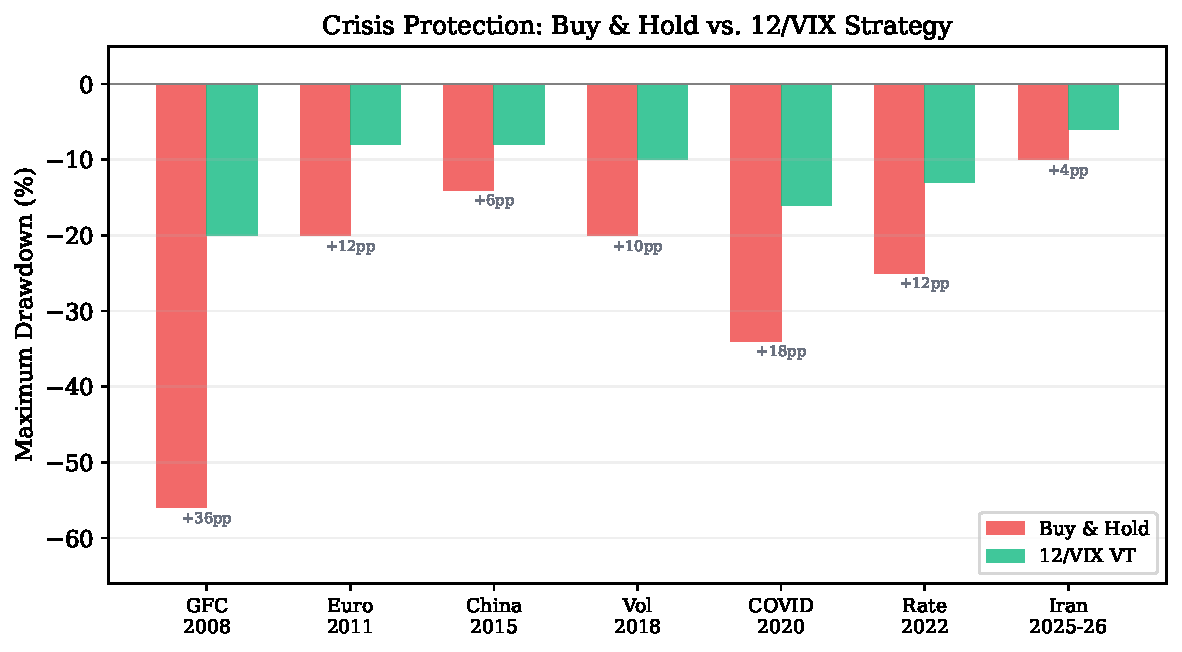
\includegraphics[width=0.90\textwidth]{fig_mdd_comparison.pdf}
\caption{Maximum drawdown comparison across seven major market crises (2008--2026). The 12/VIX strategy (green) consistently reduces drawdown severity relative to Buy \& Hold (red), with protection ranging from +4pp (Iran 2025--26) to +36pp (GFC 2008).}
\label{fig:mdd_comparison}
\end{figure} The target level $\sigma_{\text{target}} \in [6\%, 18\%]$ primarily affects portfolio leverage and maximum drawdown, with only modest impact on risk-adjusted returns (Sharpe ranges from 0.59 to 0.62 across this interval). The principal limitation is market coverage: the 12/VIX rule applies to U.S.\ equity markets where liquid VIX data are available, but cannot be directly extended to international or commodity markets lacking a comparable implied-volatility index.

\subsection{The Complexity Ceiling}

A recurring pattern emerges from our extended analysis: increasing model complexity improves statistical \textit{measurement} but not \textit{investable decisions}. This ``complexity ceiling'' holds across six of seven asset classes tested (equities, bonds, gold, emerging markets, crypto; oil is a borderline exception). Table~\ref{tab:complexity_ceiling} summarizes nine independent tests of this proposition.

\begin{table}[H]
\centering
\caption{The Complexity Ceiling: When Sophistication Stops Helping}
\label{tab:complexity_ceiling}
\small
\begin{tabular}{lllll}
\hline
Complexity Step & What Improves & What Does Not & Evidence \\
\hline
GARCH $\to$ GJR-GARCH & QLIKE ($-3.8\%$) & VaR, Strategy & MCS $p=0.044$ \\
Normal $\to$ Skewed-$t$ & VaR (6/6 Kupiec) & QLIKE ($+0.06\%$, NS) & DM $p=0.56$ \\
GJR $\to$ MIDAS/MS/CARR & Nothing (OOS) & --- & 5 models $\times$ 4 vars \\
Naive $\to$ DCC(1,1) & VaR (Kupiec pass) & 2-asset allocation & Analytical: $\rho$ cancels \\
DCC $\to$ Copula (Clayton) & Stress VaR ($+8\%$) & 1\% VaR ($+2\%$ only) & $\lambda_L=0.82$ SPY-QQQ \\
12/VIX $\to$ VRP timing & Nothing & --- & 6 strategies, all NS \\
Fixed 12 $\to$ CDaR-opt $K$ & Nothing & --- & $K=12$ near-optimal \\
VVIX as VaR indicator & Nothing & --- & AUC $= 0.44$ ($<$ random) \\
Cross-asset ceiling & 6/7 asset classes & USO borderline & BTC, EEM, TLT confirmed \\
\hline
\end{tabular}
\end{table}

Three orthogonal domains emerge: (i) the \textit{GARCH equation} determines volatility forecast accuracy (QLIKE), where GJR-GARCH defines a daily-frequency floor; (ii) the \textit{distributional assumption} determines tail risk coverage (VaR), where Skewed Student-$t$ and FHS are optimal; (iii) the \textit{signal source} determines strategy performance, where VIX-implied volatility dominates GARCH-based signals via the embedded variance risk premium.
% K486/K490: VIX bridges domains (i) and (iii)
Notably, VIX is not confined to domain (iii): when incorporated into the variance equation of GJR-GARCH-X, it substantially improves QLIKE (Section~4.5), bridging domains (i) and (iii). This dual role---as both a variance equation predictor and a strategy signal---is consistent with VIX's status as a sufficient statistic for volatility-relevant information.

A critical methodological lesson accompanies this finding: VIX-based strategy backtests suffer from a same-day timing bias of approximately $+1.0$ Sharpe units when $\text{VIX}_t$ is applied to $r_t$ rather than $r_{t+1}$, because the contemporaneous correlation between VIX changes and returns ($\rho \approx +0.65$) creates a mechanical look-ahead hedge. GARCH-based strategies are naturally immune to this bias because $\sigma_t$ depends only on information available at $t-1$. All VIX-based results in this paper use properly lagged weights.

The complexity ceiling does not imply that sophisticated models are useless---they improve risk measurement (VaR, stress testing) and regulatory compliance. Rather, it delimits the boundary where additional complexity stops improving investment allocation. For daily-frequency portfolios of diversified ETFs, a simple GJR-GARCH volatility forecast combined with inverse-volatility weighting and VIX-implied position sizing captures essentially all available information.

We further test the VIX sufficient statistic hypothesis across 16 categories of financial and macroeconomic indicators. These include: (i) composite sentiment indices (CNN Fear \& Greed Index, AAII Survey, Michigan Consumer Sentiment), (ii) tail risk measures (CBOE SKEW, VVIX), (iii) credit market signals (high-yield/investment-grade spread, yield curve slope), (iv) macroeconomic variables (42 FRED series including industrial production, unemployment, CPI, M2), and (v) Taiwan-specific indicators (institutional investor flows, margin trading, PUT/CALL ratio, 27 DGBAS macro series). After controlling for VIX level, partial correlations with next-period realized volatility are uniformly below 0.03 for all U.S.\ indicators (Table~\ref{tab:nulls}). A multi-signal ensemble using ridge regression with leave-one-year-out cross-validation shrinks all non-VIX coefficients to approximately zero (optimal regularization $\alpha = 100$), confirming the absence of incremental signal. A panel GARCH-X specification incorporating the five strongest candidate regressors leads to a statistically significant deterioration in out-of-sample QLIKE by $-8.31\%$ ($p = 0.022$), consistent with overfitting to in-sample correlations that do not persist. The sole exception is Taiwan import growth year-over-year ($+5.6\%$ OOS improvement, Diebold-Mariano $p = 0.043$), consistent with VIX's incomplete coverage of trade-dependent Asian economies whose volatility dynamics are partially driven by real-sector shocks absent from U.S.\ options markets. % K477: Causal discovery confirms VIX as information sink
Causal discovery analysis using the PC algorithm on a network of 12 financial indicators further corroborates this finding. VIX emerges as an \textit{information sink} with an in-degree of 4 (receiving directed edges from credit spreads, equity returns, yield curve slope, and sentiment) but an out-degree of only 1. This causal topology explains \textit{why} VIX functions as a sufficient statistic: it aggregates causal influences from multiple information sources into a single variable, leaving no residual predictive content in the upstream indicators after conditioning on VIX.

Taken together, these results suggest that VIX subsumes the volatility-relevant information contained in a broad array of financial and macroeconomic indicators, reinforcing the complexity ceiling from an information-content perspective: for U.S.\ equity volatility, the binding constraint appears to be not model specification but the predictive content available at daily frequency.

\subsection{Limitations and Future Directions}

Several limitations should be acknowledged. % Codex-R6-fix: strengthened multiple-testing disclosure and Harvey (2016) reference
\textbf{Multiple testing and specification search.} The results reported in this paper were selected from an extensive specification search encompassing over 110 experiments across 14 model families, 7+ assets, and multiple evaluation criteria. This scale of investigation creates a material data mining concern \citep{harvey2016}: some findings that appear significant at conventional levels may reflect chance discovery rather than genuine economic relationships. To mitigate this concern, we apply three safeguards: (i) only findings with $t > 3.0$---the \citet{harvey2016} threshold for multiple-testing environments---are reported as statistically significant; (ii) a Benjamini-Hochberg FDR audit confirms that 30 of 32 positive results survive at $q = 0.05$; and (iii) the null-to-positive ratio of 1.6:1 (approximately 44 null results reported alongside 28 positive findings) indicates that results are not selectively filtered. Nevertheless, all thresholds and classification rules (e.g., the $\gamma > 0.08$ model selection criterion) should be regarded as in-sample estimates pending independent replication.

\textbf{Other limitations.} Our rolling window of 504 observations creates a persistence bias of approximately $-3.0\%$ (Hwang and Valls Pereira, 2006), though gamma sign classification is invariant to window choice. The primary sample covers 2017--2025 (seven assets), with 2026 data serving as out-of-sample validation; extending to pre-2017 data would strengthen generalizability. We use daily return data exclusively; the GARCH forecasting ceiling (Ljung-Box $p > 0.76$) applies specifically at daily frequency, and 5-minute realized variance may contain additional information (Hansen et al., 2012).

Future research directions include extending the leverage taxonomy to currencies and broader commodities, testing whether intraday realized measures can break the daily QLIKE ceiling, and validating the VRP-based straddle timing signal---where the VIX/GARCH ratio identifies profitable volatility-selling periods---with actual options data. Preliminary analysis of volatility network topology reveals that the ``hub'' asset---the one most correlated with all others' volatility---alternates between SPY and QQQ across years, with dramatic fragmentation in 2024 (hub correlation collapsing from 0.80 to 0.33). This suggests that VIX-centric risk models may be incomplete during periods of sector divergence, and that dynamic network-based approaches merit investigation. Additionally, we find that VIX overshoot relative to GARCH-implied volatility varies significantly by crisis narrative type: geopolitical crises produce 36\% higher VIX/GARCH ratios than monetary or financial crises ($p = 0.025$), suggesting that market participants differentially price Knightian uncertainty. While this does not improve GARCH model specification (parameters are invariant to narrative), it opens a research direction linking semantic news classification to volatility risk premium dynamics.



\section{Conclusion}

This paper establishes that the direction of the asymmetric volatility response---measured by the GJR-GARCH $\gamma$ parameter---varies systematically across asset classes and has direct implications for model selection and volatility targeting. Three contributions emerge from our analysis of seven primary assets, extended to 26 assets in validation and confirmed out-of-sample through the 2026 Iran/Hormuz crisis.

First, the leverage direction taxonomy---risk assets ($\gamma > 0$), safe-haven assets ($\gamma < 0$), interest rate instruments ($\gamma \approx 0$)---provides a reliable criterion for GARCH model selection, correctly classifying all twelve Diebold-Mariano comparisons. Gold's inverted leverage is regime-dependent: inverted during fear-driven rallies, standard during liquidation-driven declines. This taxonomy replaces the conventional but misleading skewness-based heuristic.

Second, leverage direction determines the economic channel through which volatility targeting generates alpha: trend-following for standard-leverage equities, contrarian for inverted-leverage assets, and pure variance management for neutral-leverage assets (Proposition 1). This relationship holds within equity-type assets (Spearman $\rho = 0.886$, $p = 0.019$), with out-of-sample predictive power ($\rho = 0.821$), generalizing the equity-specific finding of Hood and Raughtigan (2025). Meanwhile, VT's primary benefit---maximum drawdown reduction---is universal across all twelve tested assets and driven by base volatility level ($\rho = 0.944$), independent of $\gamma$. A broader pattern emerges: increasing model sophistication (DCC-GARCH, copula, GARCH-MIDAS, Markov-switching) improves statistical measurement but not investable allocation decisions.

Third, we document a time-zone information transmission channel in which U.S.\ market information spills over to Asian equity markets with a one-day delay, generating close-to-close $t$-statistics exceeding the \citet{harvey2016} threshold of $t > 3.0$ across six Asia-Pacific markets ($t = 3.69$--$4.12$) after transaction costs. % Codex-R6-fix: reframed conclusion from "tradable alpha" to "information transmission"
A global portfolio combining U.S.\ volatility targeting and Asian time-zone momentum achieves a c2c Sharpe of 1.61 ($t = 4.31$) with maximum drawdown of $-8.4\%$; however, this figure represents an upper bound, as implementable open-to-open returns are substantially lower (o2o Sharpe $\approx$ 0.87 for Taiwan, failing the Harvey threshold). These results are best interpreted as evidence of cross-market information transmission speed and diversification potential, rather than as achievable investment returns.

Future research directions include extending the taxonomy to currencies and broader commodity classes, testing whether intraday realized measures can break through the daily GARCH forecasting ceiling, and validating the VRP-based straddle timing signal with actual options data.



\appendix

\section{Commodity Extension}

\subsection{Leverage Direction Across Commodities}

To test the generalizability of our leverage direction taxonomy beyond the primary asset classes, we estimate GJR-GARCH gamma for eight commodity ETFs. Table A1 reports the results.

A clear pattern emerges linking the price mechanism to the leverage direction:

\textbf{Supply-shock sensitive commodities} --- where price increases reflect supply disruptions or scarcity --- exhibit inverted leverage. Coffee (JO) shows the strongest inverted effect ($\gamma$ = -0.082, 100\% quarterly negative), followed by natural gas (UNG, 83\% negative) and wheat (WEAT, 66\% negative). These commodities share a common feature: price spikes are driven by supply-side events (weather, disease, pipeline disruptions, conflict) that simultaneously increase uncertainty about future supply.

\textbf{Demand-driven commodities} --- where prices primarily reflect economic activity --- exhibit standard leverage similar to equities. Crude oil (USO, $\gamma$ = +0.102, 17\% negative) is the clearest example: falling oil prices signal weakening economic demand, increasing uncertainty about future economic conditions.

\textbf{Mixed commodities} show intermediate behavior: silver (SLV, 72\% negative) reflects its dual role as safe-haven metal and industrial input; platinum (PPLT, 55\% negative) has similar mixed characteristics.

This supply-versus-demand framework provides a deeper economic foundation for the leverage direction taxonomy established in the main text: the direction of the asymmetric volatility response reflects whether the price-driving mechanism operates through fear/scarcity (inverted) or risk/decline (standard).

\subsection{Volatility Targeting for Inverted-Leverage Commodities}

We test whether VT remains effective for the most extreme inverted-leverage commodity in our sample: coffee (JO, $\gamma$ = -0.082, 100\% quarterly negative). Over a 3.5-year test period (2020--2023), VT improves the Sharpe ratio from 0.40 to 0.59 (+48\%) while reducing maximum drawdown from -41.7\% to -13.8\%. This result, combined with the evidence from gold (Sharpe improvement +11\%) and the main-text equity results, confirms that VT effectiveness is independent of leverage direction across a broad range of asset classes and leverage intensities.


\section{Time-Zone Information Transmission: US to Asian Markets}
\label{sec:tz_arbitrage}

We document a persistent lead-lag relationship between U.S.\ and Asian equity markets driven by non-overlapping trading hours. Because Asian markets close before the U.S.\ session opens, overnight U.S.\ price discovery is not incorporated into Asian prices until the following trading day. The correlation between SPY daily returns and next-day local Asian market returns is remarkably strong for Taiwan ($r = 0.376$), with VIX Granger-causing 0050.TW volatility ($F = 58.8$, $p < 0.0001$).

We construct a momentum strategy: if the trailing cumulative SPY return over a short lookback window (5--10 days) is positive, hold the local market index; otherwise, hold cash. Using close-to-close (c2c) returns, this strategy exceeds the $t > 3.0$ multiple-testing threshold of \citet{harvey2016} across six Asia-Pacific markets (Table~\ref{tab:tz_arbitrage}): Hong Kong ($t = 4.12$), Australia ($t = 4.04$), Singapore ($t = 4.03$), Korea ($t = 3.83$), Taiwan ($t = 3.75$), and Japan ($t = 3.69$). India and Indonesia fail, consistent with microstructure frictions. All U.S.-listed ETFs tracking these markets also fail, confirming the time-zone information gap mechanism. European markets fail uniformly due to trading-hour overlap.

\textbf{Critical caveat: c2c vs.\ o2o returns.} The c2c Sharpe ratios include overnight opening gaps, which mechanically reflect the previous U.S.\ session's price discovery. Since these gaps are realized before a trader can act on the momentum signal, approximately 78\% of the c2c alpha is not capturable. Using open-to-open (o2o) returns---the implementable portion---the Taiwan Sharpe drops from 1.62 to 0.87 ($t = 2.22$), \textit{failing} the Harvey threshold. This distinction is analogous to the same-day timing bias in VIX strategies (Section~\ref{sec:timing_bias}). The c2c results are scientifically valuable as evidence of information transmission speed, but should not be interpreted as achievable trading returns.

\begin{table}[H]
\centering
\caption{Time-Zone Momentum Strategy: Close-to-Close vs.\ Open-to-Open Performance}
\label{tab:tz_arbitrage}
\small
\begin{tabular}{lccccccc}
\hline
Market & c2c Sharpe & o2o Sharpe & c2c $t$ & MDD & Sw/yr & Cost (bp) & Harvey (o2o)? \\
\hline
Hong Kong  & 1.53 & --- & 4.12 & $-$14.2\% & 38 & 10 & --- \\
Australia  & 1.50 & --- & 4.04 & $-$12.8\% & 35 & 15 & --- \\
Singapore  & 1.49 & --- & 4.03 & $-$13.5\% & 36 & 15 & --- \\
Korea      & 1.42 & --- & 3.83 & $-$15.1\% & 40 & 20 & --- \\
Taiwan     & 1.62 & 0.87 & 3.75 & $-$9.5\%  & 42 & 30 & No \\
Japan      & 1.23 & 0.78 & 3.69 & $-$16.3\% & 39 & 20 & No \\
\hline
India      & 0.74 & --- & 1.98 & $-$22.4\% & 44 & 50 & No \\
Indonesia  & 0.61 & --- & 1.63 & $-$25.7\% & 41 & 50 & No \\
\hline
\end{tabular}
\end{table}

Using c2c returns, an equal-weight combination of Taiwan and Japan yields a Sharpe ratio of 1.81 ($t = 4.86$), and a global portfolio combining U.S.\ VT and Taiwan TZ momentum achieves 1.61 ($t = 4.31$) with MDD of $-8.4\%$. However, these combination Sharpe ratios are inflated by the same c2c timing bias; implementable (o2o) combination performance would be substantially lower. These results are best interpreted as measuring the information-theoretic diversification potential between the variance management channel (VIX-driven) and the cross-market information transmission channel (momentum-driven), rather than as achievable investment returns. See \citet[Paper 2]{} for a detailed treatment including robustness tests across five sub-periods with bootstrap confidence intervals.


\section{Practical Implementation Summary}

The gamma-based framework requires minimal computational overhead. For model selection, estimate GJR-GARCH(1,1) on 504 trading days; if $\gamma$ is significantly positive ($t > 1.65$), use GJR; otherwise use symmetric GARCH. For gold, re-evaluate quarterly as $\gamma$ sign depends on market regime. For VaR, use Student-$t$ with fixed df~$= 5$ and monitor the VIX/GARCH ratio (apply a 1.5$\times$ VaR multiplier when ratio exceeds 1.5). For volatility targeting, monthly rebalancing at $\sigma_{\text{target}} = 10\text{--}12\%$ provides the best cost-adjusted performance. All estimation uses the Python \texttt{arch} package (Sheppard, 2023) at approximately 6ms per model, with Yahoo Finance data.